%%________________________________________________________________________
%% LEIM | PROJETO
%% 2022 / 2013 / 2012
%% Modelo para relatório
%% v04: alteração ADEETC para DEETC; outros ajustes
%% v03: correção de gralhas
%% v02: inclui anexo sobre utilização sistema controlo de versões
%% v01: original
%% PTS / MAR.2022 / MAI.2013 / 23.MAI.2012 (construído)
%%________________________________________________________________________
%%
%%
%% É importante ver o essencial do LaTeX antes de usar este template.
%% um bom "ponto de partida": http://en.wikibooks.org/wiki/LaTeX/
%%
%%________________________________________________________________________
%% Para alterar o Título, Nome dos Autores e Nome dos Orientadores fazer:
%% - abrir o ficheiro "00_PRJ_padrao.sty"
%% - procurar "Nome do aluno" e alterar
%% - procurar "número" e alterar; deixar os parêntesis
%% - procurar "Nome do orientador" e alterar
%% - procurar "[Doutor]" e atirar os parêntesis rectos ou eliminar tudo
%%
%% Caso precise de adicionar um novo aluno, ou orientador, deve:
%% - selecionar toda a linha (com "Nome do aluno" ou "Nome do orientador")
%% - seleccionar a linha imediatamente acima dessa
%% - copiar ambas as linhas
%% - colocar as linhas copiadas logo abaixo da primeira linha seleccionada
%%________________________________________________________________________





%% o documento é definido do tipo "book" em a4, font 12pt
\documentclass[a4paper,12pt]{book}

\usepackage[acronym, nomain]{glossaries}
\makeglossaries


%% para usar caracteres acentuados
\usepackage[utf8]{inputenc} % no Unix (com codificação UTF-8)
%% \usepackage[latin1]{inputenc} % no Windows (com codificação ISO-8859-1, ou ISO-8859-15)

% para aspectos de hifenização (do Português)
\usepackage[portuguese]{babel}

%% para incluir imagens e tratar de modo adequado endereços url
\usepackage{graphicx,url}

%% para usar \begin{comment} ... \end{comment}
\usepackage{verbatim}

%% para usar o símbolo do euro
%usepackage{eurosym}

%% para juntar multiplas linhas em tabelas
\usepackage{multirow}

%% para usar símbolos matemáticos
\usepackage[centertags]{amsmath}

%% para usar \mathds{...}
\usepackage{dsfont}

%% para formatação (e.g. espaçamento) de Tabelas
\usepackage{tabls}

%% para usar listagens de código
\usepackage{listings}

%% para escrita "formal" de algoritmos
\usepackage{algorithm}

%% Para que a numeracao de listings seja global
%% (e nao no contexto de cada capitulo!)
\usepackage{chngcntr}

% para usar um estilo diferente na identificação de "Capítulo"
%Sonny, Lenny(x), Glenn, Conny, Rejne, Bjarne
%\usepackage[Lenny]{fncychap}
% Para ter no "heading" o nome do capítulo e da secção
\usepackage{fancyhdr}



% para usar hiperligações (especialmente relevante para o índice)
\usepackage[hidelinks]{hyperref}
%\hypersetup{linktocpage}
%\hypersetup{
%    colorlinks,
%    citecolor=black,
%    filecolor=black,
%    linkcolor=black,
%    urlcolor=black
%}

%%________________________________________________________________________
%% para incluir o estilo proposto
\usepackage{./00_PRJ_padrao}
%%________________________________________________________________________



%%________________________________________________________________________
% mudar alguns nomes fixos para Português
%%________________________________________________________________________
% renomear "Listing" para "Código"
\renewcommand{\lstlistingname}{Código}
\addto\captionsportuges{
    \renewcommand{\contentsname}{Apêndice}}
\addto\captionsportuges{
    \renewcommand{\bibname}{Bibliografia}}
\addto\captionsportuges{
    \renewcommand{\proofname}{Prova}}
\addto\captionsportuges{
    \renewcommand{\chaptername}{Capítulo}}
\setlength{\headheight}{15pt}

\newcommand{\myListOfAcronymns}{
    \cleardoublepage
    \phantomsection
    \addcontentsline{toc}{chapter}{Lista de Acrónimos}
    \printglossary[type=\acronymtype, title=Lista de Acrónimos]
}
%%________________________________________________________________________

\newacronym{vscode}{VSCode}{Visual Studio Code}
\newacronym{csv}{CSV}{Comma-Separated Values}
\newacronym{ui}{UI}{User Interface}
\newacronym{ux}{UX}{User Experience}
\newacronym{api}{API}{Application Programming Interface}
\newacronym{xlsx}{XLSX}{Excel Spreadsheet Format}
\newacronym{iscal}{ISCAL}{Instituto Superior de Contabilidade e Administração de Lisboa}
\newacronym{isel}{ISEL}{Instituto Superior de Engenharia de Lisboa}
\newacronym{captcha}{CAPTCHA}{Completely Automated Public Turing test to tell Computers and Humans Apart}
\newacronym{sad}{SAD}{Sistemas de Apoio à Decisão}
\newacronym{uml}{UML}{Unified Modeling Language}
\newacronym{etl}{ETL}{Extract, Transform, Load}
\newacronym{mvc}{MVC}{Model-View-Controller}
\newacronym{orm}{ORM}{Object-Relational Mapping}
\newacronym{sql}{SQL}{Structured Query Language}
\newacronym{crm}{CRM}{Customer Relationship Management}
\newacronym{cms}{CMS}{Content Management System}
\newacronym{json}{JSON}{JavaScript Object Notation}
\newacronym{html}{HTML}{HyperText Markup Language}
\newacronym{css}{CSS}{Cascading Style Sheets}
\newacronym{js}{JS}{JavaScript}
\newacronym{dom}{DOM}{Document Object Model}
\newacronym{spa}{SPA}{Single Page Application}
\newacronym{wsgi}{WSGI}{Web Server Gateway Interface}
\newacronym{uuid}{UUID}{Universally Unique Identifier}
\newacronym{uc}{UC}{Use Case}
\newacronym{http}{HTTP}{Hypertext Transfer Protocol}~
\newacronym{wcag}{WCAG}{Web Content Accessibility Guidelines}
\newacronym{cli}{CLI}{Command Line Interface}
\newacronym{seo}{SEO}{Search Engine Optimization}
\newacronym{gzip}{GZIP}{GNU Zip}
\newacronym{aria}{ARIA}{Accessible Rich Internet Applications}
\newacronym{rest}{REST}{Representational State Transfer}
%% \acfoot{dom}
%% \gls{dom}

%%________________________________________________________________________
%%%%%%%%%%%%%%%%%%%%%%%%%%%%%%%%%%%%%%%%%%%%%%%%%%%%%%%%%%%%%%%%%%%%%%%%%%
%% Begin Document
%%%%%%%%%%%%%%%%%%%%%%%%%%%%%%%%%%%%%%%%%%%%%%%%%%%%%%%%%%%%%%%%%%%%%%%%%%
\begin{document}
% para que a numeracao de listings seja global
% (e nao no contexto de cada capitulo!)
\counterwithout{lstlisting}{chapter}
%% incluir a capa
\frontmatter
\fazerCapa
%% incluir o resumo e abstract
%% caso pretenda, incluir os agradecimentos e a dedicatória
\frontmatter
%%________________________________________________________________________
%% comentar o que não interessar
%%________________________________________________________________________
%% LEIM | PROJETO
%% 2022 / 2013 / 2012
%% Modelo para relatório
%% v04: alteração ADEETC para DEETC; outros ajustes
%% v03: correção de gralhas
%% v02: inclui anexo sobre utilização sistema controlo de versões
%% v01: original
%% PTS / MAR.2022 / MAI.2013 / 23.MAI.2012 (construído)
%%________________________________________________________________________




%%________________________________________________________________________
\myPrefaceChapter{Resumo}
%%________________________________________________________________________

Neste trabalho apresentamos o desenvolvimento de uma aplicação \textit{web} para visualização de dados, pensada para facilitar a análise da informação exportada da plataforma \textit{International Corporate Management} da empresa \textit{Marketplace Simulations}, usada na unidade curricular Projeto de Simulação em Negócios Internacionais, lecionada na Licenciatura em Comércio e Negócios Internacionais do ISCAL.

A motivação principal surgiu da ausência de visualizações integradas na plataforma, que dificulta a leitura dos dados, mas que permite exportar vários ficheiros \textit{Excel} com a informação necessária. Assim, o objetivo da nossa aplicação passa por permitir aos alunos carregar os ficheiros exportados, e visualizar os resultados através de gráficos, reduzindo o esforço manual e aumentando a clareza dos dados.

A solução foi organizada com base nos períodos de simulação da plataforma de simulação, permitindo ao utilizador agrupar e consultar os dados por fase. Cada ficheiro carregado passa por uma \textit{pipeline} de tratamento de dados implementada em \textit{Python} utilizando a biblioteca \textit{Pandas}. Os gráficos são feitos com recurso à biblioteca \textit{Plotly}, integrada na interface gráfica da aplicação.

A aplicação foi desenvolvida com \textit{Django}, onde foi implementada toda a lógica de servidor. A interface visual utiliza as bibliotecas \textit{Flowbite}, \textit{Plotly} e \textit{Datatables}, que garantem uma interface intuitiva e responsiva. A aplicação foi construída de forma incremental e modular, e encontra-se preparada para múltiplos utilizadores.

Como resultado, a aplicação desenvolvida facilita a leitura dos dados. A solução contribuiu para uma análise mais acessível e interativa, apoiando a tomada de decisões em contexto académico.

%%________________________________________________________________________
\myPrefaceChapter{Abstract}
%%________________________________________________________________________

In this paper, we present the development of a web application for data visualization, designed to facilitate the analysis of information exported from the International Corporate Management platform of Marketplace Simulations, used in the International Business Simulation Project course, taught in the Bachelor's Degree in International Trade and Business at ISCAL.

The main motivation arose from the absence of integrated visualizations in the platform, which makes it difficult to read the data, but allows several Excel files with the necessary information to be exported. Thus, the goal of our application is to allow students to upload the exported files and view the results through graphs, reducing manual effort and increasing data clarity.

The solution was organized based on the simulation periods of the simulation platform, allowing the user to group and consult the data by phase. Each uploaded file goes through a data processing pipeline implemented in Python using the Pandas library. The graphs are made using the Plotly library, integrated into the application's graphical interface.

The application was developed with Django, where all server logic was implemented. The visual interface uses the Flowbite, Plotly, and Datatables libraries, which ensure an intuitive and responsive interface. The application was built incrementally and modularly and is ready for multiple users.

As a result, the developed application facilitates data reading. The solution contributed to a more accessible and interactive analysis, supporting decision-making in an academic context.
%%________________________________________________________________________
%% LEIM | PROJETO
%% 2022 / 2013 / 2012
%% Modelo para relatório
%% v04: alteração ADEETC para DEETC; outros ajustes
%% v03: correção de gralhas
%% v02: inclui anexo sobre utilização sistema controlo de versões
%% v01: original
%% PTS / MAR.2022 / MAI.2013 / 23.MAI.2012 (construído)
%%________________________________________________________________________




%%________________________________________________________________________
\myPrefaceChapter{Agradecimentos}
%%________________________________________________________________________

Ao longo do desenvolvimento deste projeto, tive a oportunidade de contar com a orientação de docentes do ISEL e do ISCAL, a quem agradeço pelo o apoio dado durante o projeto. 

Ao Professor Artur Ferreira (ISEL), Paulo Trigo (ISEL) e  Professor Hélder Fanha (ISCAL), que, em diferentes momentos, contribuíram com sugestões, comentários e sugestões. O seu acompanhamento ajudou a resolver dúvidas que surgiram durante o desenvolvimento, e a validar algumas das opções técnicas.

Fica aqui, então, o meu agradecimento pelo contributo dado ao longo deste processo.

%%________________________________________________________________________
%% LEIM | PROJETO
%% 2022 / 2013 / 2012
%% Modelo para relat�rio
%% v04: altera��o ADEETC para DEETC; outros ajustes
%% v03: corre��o de gralhas
%% v02: inclui anexo sobre utiliza��o sistema controlo de vers�es
%% v01: original
%% PTS / MAR.2022 / MAI.2013 / 23.MAI.2012 (constru�do)
%%________________________________________________________________________




%%________________________________________________________________________
\begin{myDedication}
%%________________________________________________________________________

Eventual texto de dedicat�ria \ldots

\vskip0.4in
\ldots mais texto,

\vskip0.8in
\ldots e o fim do texto.
    
    
\end{myDedication}
%%________________________________________________________________________

%% incluir a lista de conteúdos (índice, tabelas e figuras)
%comentar se quiser alterar o espaçamento entre linhas
\setlinespacing{1.15}
\myTableOfContents
%%________________________________________________________________________
%% comentar o que não interessar

\myListOfTables
\myListOfFigures
\myListOfAcronymns
%%________________________________________________________________________





%% "Corpo Principal" do texto
\mainmatter
\myPageStyle

No sistema, o \gls{csv} pe
%% cada um dos Capítulos
%% (aqui separados em dois ficheiros)
%%________________________________________________________________________
%% comentar o que não interessar (ou incluir outros ficheiros)
%%________________________________________________________________________
%% LEIM | PROJETO
%% 2022 / 2013 / 2012
%% Modelo para relatório
%% v04: alteração ADEETC para DEETC; outros ajustes
%% v03: correção de gralhas
%% v02: inclui anexo sobre utilizaçãa aplicação controlo de versões
%% v01: original
%% PTS / MAR.2022 / MAI.2013 / 23.MAI.2012 (construído)
%%________________________________________________________________________


%%________________________________________________________________________
\chapter{Introdução}
\label{ch:introducao}
%%________________________________________________________________________

No contexto do ensino superior, tem-se dado cada vez mais importância à integração de ferramentas tecnológicas que tornem o processo de aprendizagem mais prático, como é o caso do simulador utilizado pelos alunos do \gls{iscal}. Esta ferramenta permite que os estudantes apliquem, de forma interativa, os conhecimentos adquiridos ao longo do curso, colocando-os em situações de tomada de decisão semelhantes às que enfrentariam num ambiente real. Deste modo, o simulador não só reforça os conteúdos teóricos, como também reforça o desenvolvimento das competências aprendidas. 

Neste contexto, a análise eficiente de dados torna-se essencial para a tomada de decisões e tem impacto na avaliação final dos alunos, no entanto, a complexidade e a falta de uma ferramenta visual que ajude a perceber as informações apresentadas pode representar um desafio grande para os estudantes.

\section{Motivação}

O presente projeto surgiu da necessidade  entre os alunos do \gls{iscal} que utilizam o simulador \textit{Marketplace Simulations - International Corporate Management}, que é um simulador de negócios internacionais e que iremos descrever no capítulo (cf. capítulo~\ref{sec:marketplace}), onde os alunos se agrupam em empresas e simulam a criação de um negócio num mercado internacional. Embora a plataforma apresente toda a informação necessária à tomada de decisões na simulação, esses dados estão divididos em múltiplas secções e apresentados em tabelas, com poucas funcionalidades de visualização. Esta limitação obriga os alunos a alternar entre páginas, copiar dados manualmente e criar folhas de cálculo externas, comprometendo a eficiência e a análise da informação.

\section{Objetivos}

A aplicação proposta neste relatório pretende ajudar nesse sentido, oferecendo uma interface que permite aos utilizadores carregar dados retirados da plataforma de simulação e tornar esses ficheiros em visualizações que podem ser consultadas e manipuladas. A aplicação permitirá aos utilizadores:

\begin{itemize}
    \item Criar uma conta na plataforma que suporte a persistência da informação carregada.
    \item Carregar ficheiros exportados da plataforma de simulação.
    \item Visualizar os dados em gráficos interativos.
    \item Conseguir ter uma experiência de utilização intuitiva e fácil.
\end{itemize}

Pretende-se também que a aplicação adote uma arquitetura simples de manter e que utilize os mesmos conceitos que a plataforma de simulação, dando importância aos seguintes itens:

\begin{itemize}
    \item A normalização e transformação automática de dados carregados.
    \item A facilidade na gestão de ficheiros, com o objetivo de oferecer uma interface fácil para os utilizadores finais.
    \item Organizar a informação por utilizador, garantindo que o utilizador apenas consegue consultar a informação carregada.
    \item Adotar um modelo de funcionamento semelhante à plataforma de simulação, de modo a tornar a experiência de utilização mais intuitiva e garantido que a nossa aplicação tenha fronteiras claras de utilização.
\end{itemize}

Ao longo deste relatório, serão apresentadas as decisões tomadas, bem como os fundamentos que orientaram o desenvolvimento da aplicação proposta.

%%________________________________________________________________________
\chapter{Trabalho Relacionado}
\label{ch:trabalhoRelacionado}
%%________________________________________________________________________

O presente projeto insere-se num contexto mais geral de ferramentas pedagógicas e de \gls{sad}, ainda que neste caso concreto, em ambientes simulados no ensino superior. No âmbito do \gls{iscal}, a utilização da plataforma \textit{Marketplace Simulations} \cite{MarketplaceSim_2025} permite aos estudantes desenvolver competências práticas em ambientes virtuais de negócios, simulando o funcionamento de mercados reais. A necessidade de suporte digital à análise e simulação motivou o desenvolvimento de outras ferramentas auxiliares, com destaque para um projeto também realizado em parceria com o \gls{iscal}, focado em simulações parciais de modelos económicos.

Esse projeto, embora partilhe uma motivação semelhante, segue uma abordagem diferente. Em particular, a aplicação referida acima permite simular cenários específicos com base em \textit{inputs} manuais, o que pode ser útil para quando se procura prever resultados com foco muito concreto (por exemplo, simular o impacto de uma única variável nos resultados). A nossa plataforma foca-se numa outra vertente, em que pretende ser uma ferramenta para auxiliar o ensino de forma prática.

O projeto assume então o uso de dados extraídos diretamente da plataforma de simulação, e a valorização da experiência do utilizador na apresentação de dados. Não será uma plataforma de simulação, mas sim uma ferramenta para auxiliar o ensino de forma prática.

\textbf{Sistemas de apoio à decisão}
\label{sec:sad}

Um \gls{sad} é uma aplicação, ou um conjunto de aplicações, concebida para auxiliar utilizadores na tomada de decisões mais informadas e fundamentadas. Ao contrário de sistemas automatizados que tomam decisões de forma autónoma, um \gls{sad} funciona como uma ferramenta que mostra aos utilizadores os dados e análises necessárias para que estes possam avaliar alternativas, prever resultados e escolher a melhor ação possível.

Na prática, um \gls{sad} é responsável por recolher, organizar e processar grandes volumes de dados, muitas vezes com origem em múltiplas fontes, e transformá-los em informação relevante. Esta informação é normalmente apresentada através de tabelas, indicadores ou representações visuais como gráficos de barras, linhas, setores ou até mapas interativos. Um aspeto importante é a capacidade de aplicar filtros e explorar diferentes cenários, o que permite ao utilizador testar hipóteses, identificar padrões e comparar opções de forma mais eficiente.

Estes sistemas são particularmente úteis em contextos onde há grande complexidade ou incerteza, por exemplo, na gestão empresarial, em análises financeiras, em planeamento estratégico, ou na análise de mercados. Num ambiente académico ou de simulação, como é o caso da plataforma usada neste projeto, um \gls{sad} ajuda os estudantes a perceber melhor o impacto das suas decisões, mostrando dados históricos e tendências que possam não ser muito visíveis numa visualização mais básica.

É importante reforçar que o \gls{sad} não substitui o elemento humano. Em vez disso, potencia a capacidade do utilizador de interpretar a informação disponível e tomar decisões com base em evidência, reduzindo o risco de erro e aumentando a confiança no processo de decisão. Estes sistemas podem ser plataformas criadas especificamente para o efeito, ou podem ser derivadas de outras plataformas como PowerBI, Tableau, Grafana, ou outras ferramentas de visualização de dados.

%%________________________________________________________________________
\chapter{Modelo Proposto}
\label{ch:modeloProposto}
%%________________________________________________________________________

Neste capítulo descrevemos o modelo que serviu de base à implementação da aplicação, com foco na forma como os dados são organizados, processados e apresentados ao utilizador. A estrutura proposta resulta diretamente das necessidades identificadas durante a análise dos ficheiros obtidos da plataforma de simulação, bem como dos requisitos definidos com os orientadores do projeto.

O modelo tem como objetivo garantir que a aplicação desenvolvida corresponde as necessidades identificadas. Para isso, foram definidos vários componentes principais, incluindo a forma como os ficheiros são organizados por trimestre, as transformações aplicadas aos dados entre outras decisões que foram tomadas durante o desenvolvimento do projeto.

Nos próximos parágrafos vamos então detalhar cada uma das partes do modelo proposto, estabelecendo também os requisitos funcionais e não funcionais que foram definidos para a aplicação.

%%________________________________________________________________________
\section{Requisitos}
\label{sec:requisitos}
%%________________________________________________________________________

\subsubsection{Requisitos funcionais}

Os requisitos funcionais descrevem as funcionalidades específicas que a aplicação deve oferecer para atender às necessidades dos utilizadores. No contexto deste projeto, definem as ações que a aplicação deve ser capaz de executar.

Em suma, para o projeto, identificamos os seguintes requisitos, ordenados por prioridade. Os tabelas de requisitos por inteiro, incluindo algumas definições adicionais, estão incluidas em apêndice (\cf, apêndice \ref{ch:tabRequisitos}).

\begin{itemize}
    \item \textbf{Visualização de dados:} os utilizadores devem poder visualizar gráficos interativos baseados nos dados carregados, com a possibilidade de aplicar filtros como país ou \textit{quarter} selecionado.

    \item \textbf{Gestão de ficheiros:} os utilizadores devem poder carregar ficheiros, associá-los a \textit{quarters} e eliminá-los quando necessário. a aplicação valida os formatos e garante que apenas ficheiros válidos são processados.
    
    \item \textbf{Gestão de \textit{quarters}:} cada utilizador pode criar períodos identificados como \textit{Quarter N}, para organizar os ficheiros carregados. Tem também de ser possível visualizar a lista de \textit{quarters} disponíveis.

    \item \textbf{Autenticação:} a aplicação deve permitir a criação de contas e o \textit{login} por parte dos utilizadores, garantindo que cada um acede apenas aos seus próprios dados.

    \item \textbf{Normalização de dados:} os dados extraídos dos ficheiros devem ser automaticamente normalizados para garantir consistência e compatibilidade com a aplicação de visualização.
    
\end{itemize}

\subsubsection{Requisitos não funcionais}

Alguns requisitos não funcionais foram igualmente críticos para garantir a estabilidade e a capacidade de interação da aplicação. Os requisitos identificados foram os seguintes:

\begin{itemize}
    \item \textbf{Usabilidade:} a aplicação deve ser intuitiva, suportar múltiplos \textit{browsers} e permitir o carregamento progressivo de gráficos sem bloquear a interface visual (\textit{lazy load}).
    
    \item \textbf{Performance:} a aplicação deve ser capaz de suportar múltiplos utilizadores em simultâneo, mantendo uma resposta rápida às interações.
    
    \item \textbf{Acessibilidade:} a aplicação \textit{web} deve ser acessível por teclado e compatível com leitores de ecrã (\textit{screen-reader friendly}).

\end{itemize}

\section{Casos de Utilização}
\label{ch:casosUtilizacao}

Com base nos requisitos funcionais e não funcionais identificados na secção anterior, foram definidos os casos de utilização que iremos suportar. A figura~\ref{fig:umlCasosUtilizacao} apresenta o diagrama UML de casos de utilização da aplicação desenvolvida. Este diagrama ilustra as principais interações entre o utilizador e a aplicação, bem como a forma como diferentes componentes externos, nomeadamente a base de dados e a aplicação de ficheiros, participam nas operações principais da plataforma.

\begin{figure}[h]
\centering
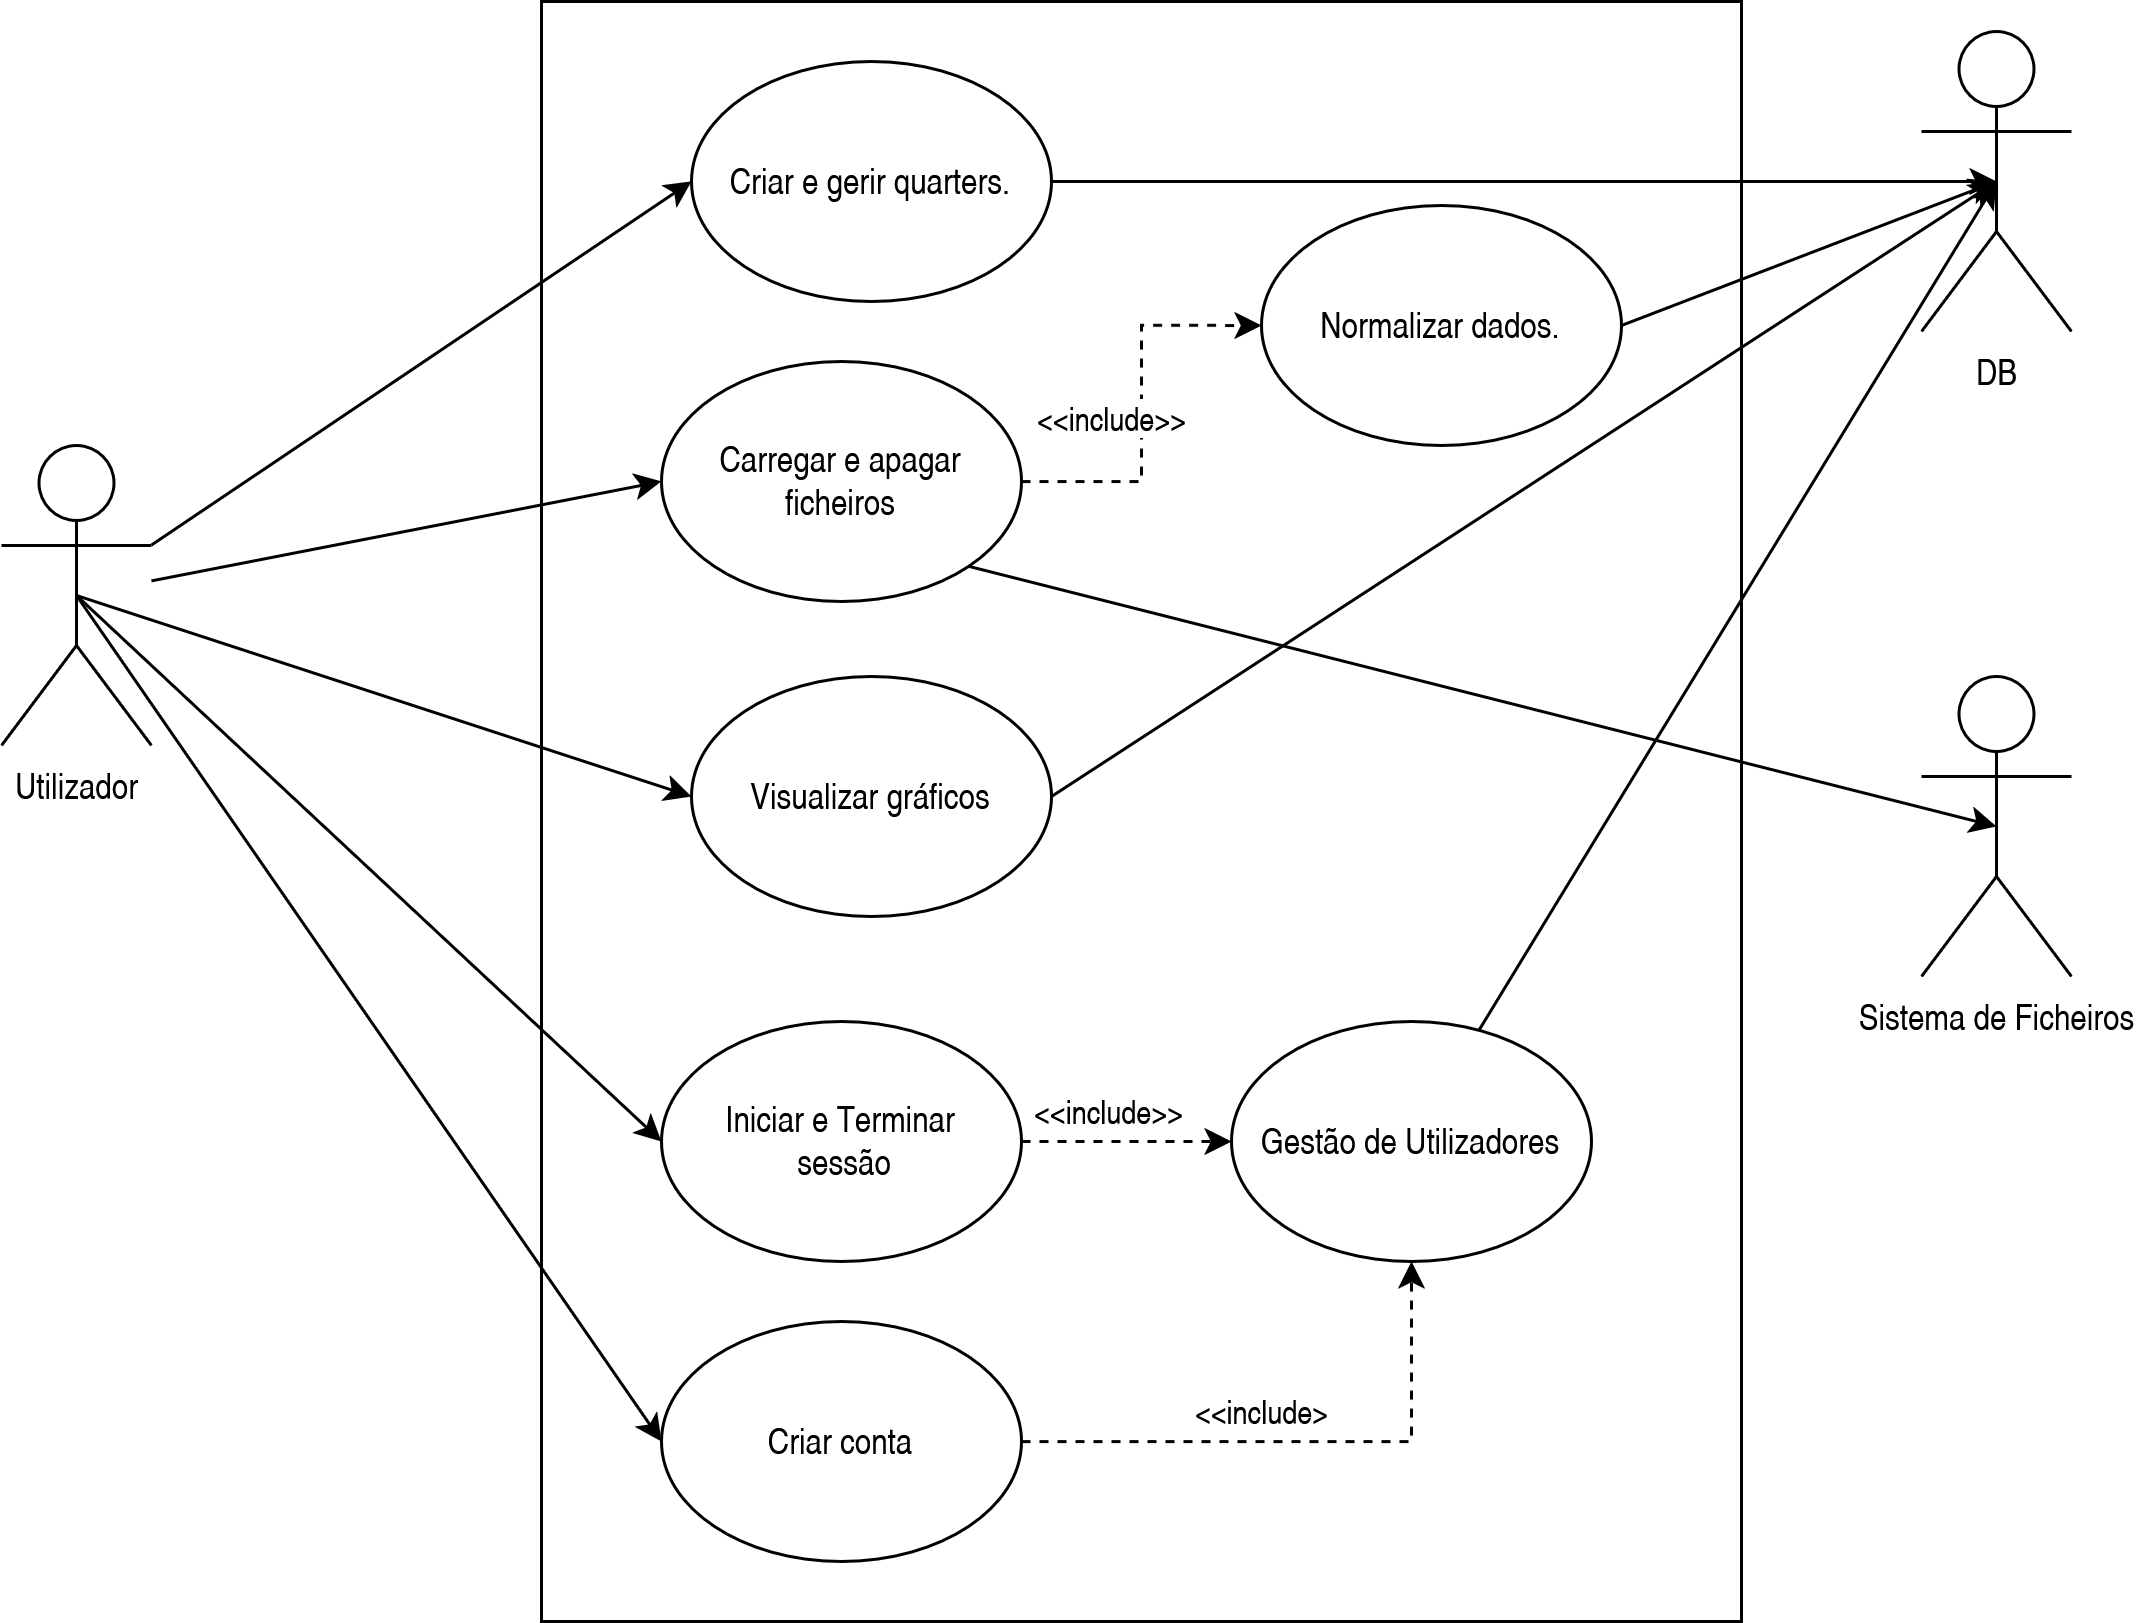
\includegraphics[max width=\textwidth]{./img/usecase_uml}
\caption{\gls{uml} dos Casos de Utilização}
\label{fig:umlCasosUtilizacao}
\end{figure}

\subsection{Atores}
\begin{itemize}
    \item \textbf{Utilizador} É o ator principal, responsável por interagir com a aplicação. Pode criar conta, iniciar sessão, carregar ficheiros, visualizar gráficos, entre outras ações.
    \item \textbf{DB (Base de Dados)} Responsável por armazenar dados, incluindo utilizadores, trimestres, ficheiros processados e metadados associada.
    \item \textbf{Sistema de Ficheiros} Componente responsável pelo armazenamento físico dos ficheiros carregados.
\end{itemize}

\subsection{Casos de Utilização}
\begin{itemize}
    \item \textbf{Criar e gerir \textit{quarters}}
    Permite ao utilizador, após autenticação, criar \textit{quarters}. Cada \textit{quarter} é identificado por um número (único por utilizador) e guardado na base de dados, sendo associado a um \gls{uuid} para efeitos internos.

    \item \textbf{Carregar ficheiros} O utilizador seleciona um \textit{quarter} e carrega ficheiros exportados da plataforma de simulação. a aplicação valida os ficheiros, extrai e processa cada folha de cálculo e aplica a \textit{pipeline} de normalização. Os dados normalizados são armazenados e associados ao \textit{quarter} correspondente.

    \item \textbf{Eliminar ficheiros} Permite ao utilizador remover ficheiros previamente carregados. a aplicação atualiza os registos no backend, marca os dados antigos como inativos e evita que sejam considerados nos gráficos, garantindo que apenas uma versão está ativa por ficheiro.

    \item \textbf{Normalizar dados} (\textit{include}) Sub-processo automático executado durante o carregamento de ficheiros. Converte os dados para um formato estruturado (por exemplo, CSV), elimina colunas irrelevantes, ajusta nomes e assegura consistência. Comunica com a base de dados e a aplicação de ficheiros.

    \item \textbf{Consultar gráficos} Após o carregamento dos ficheiros, o utilizador pode consultar gráficos com base nos dados normalizados. A aplicação permite aplicar filtros, navegar entre \textit{quarters} e visualizar apenas os dados mais recentes, garantindo performance e clareza.

    \item \textbf{Criar conta} Permite o registo de novos utilizadores. A aplicação valida os dados inseridos, verifica se o utilizador já existe e cria a conta, autenticando automaticamente o utilizador após sucesso.

    \item \textbf{Permitir \textit{login} de utilizador} O utilizador introduz credenciais válidas (\textit{username} e \textit{password}) e, caso sejam corretas, é autenticado e redirecionado para a interface principal. Este processo inclui a gestão da sessão.

\end{itemize}

% Em suma, queremos que a aplicação seja capaz de ser utilizada de acordo com o diagrama \ref{fig:flowchart}.

% \begin{figure}[H]
%     \centering
%     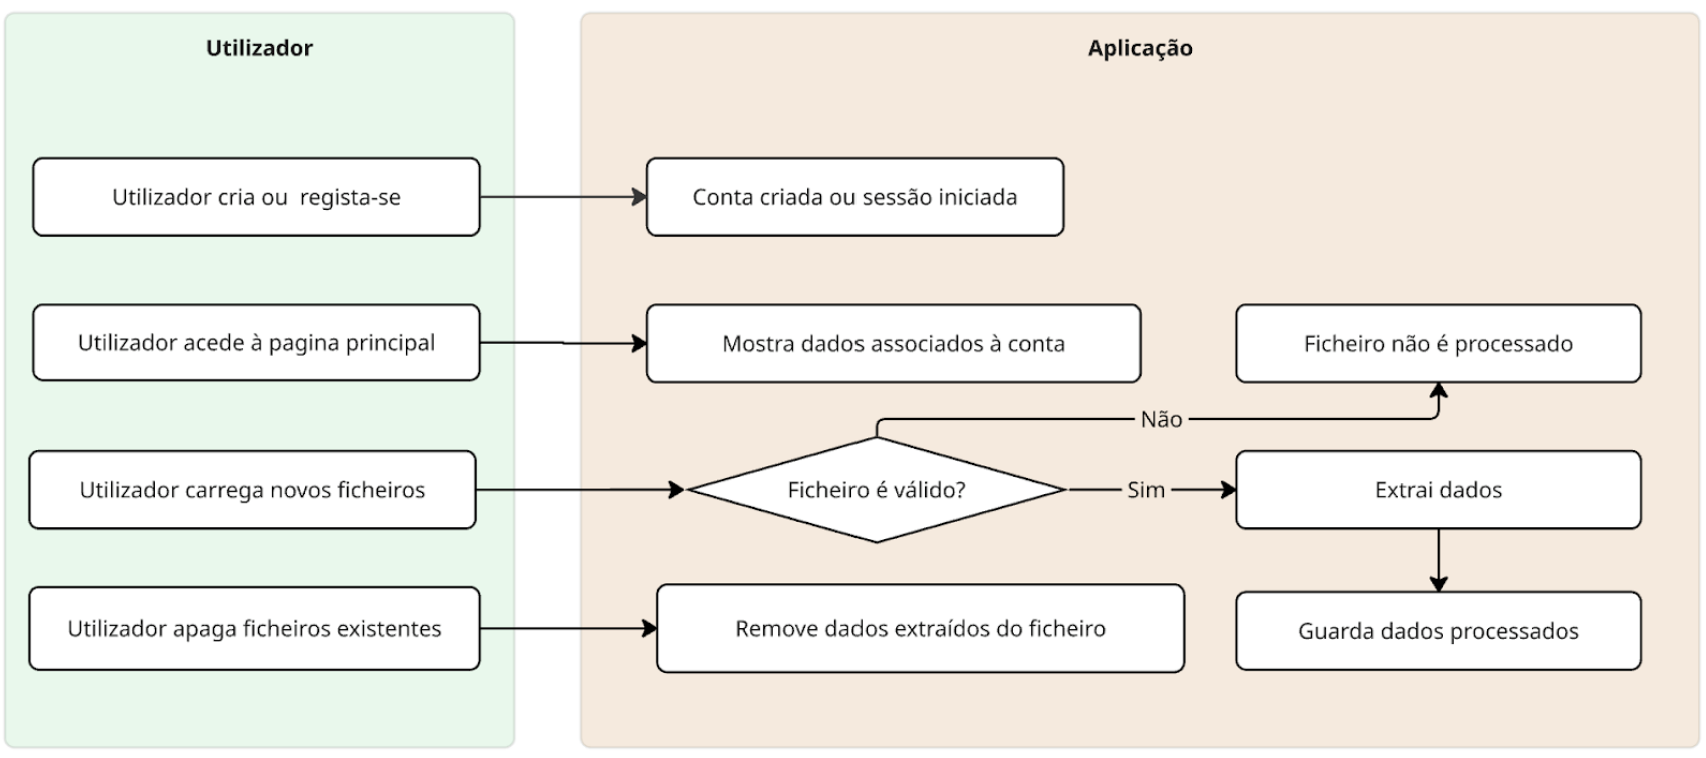
\includegraphics[max width=\textwidth]{./img/flowchart.png}
%  \caption{Diagrama de fluxo da aplicação}
%  \label{fig:flowchart}
%  \end{figure}

%%________________________________________________________________________
\section{Fundamentos}
\label{sec:fundamentos}

Neste capitulo iremos descrever as bases nas quais fundamentamos o projeto, e algumas noções necessárias para conseguir contextualizar as decisões tomadas.

\subsection{\textit{Marketplace Simulations}}
\label{sec:marketplace}

A \textit{Marketplace Simulations} \cite{MarketplaceSim_2025} é uma empresa que desenvolve plataformas de simulação para fins educativos, ou seja, ferramentas que colocam os estudantes numa espécie de jogo onde cada equipa gere a sua própria empresa e compete com os colegas em cenários simulados. Acabam então por funcionar como laboratórios virtuais que podem ser usados no ensino superior, onde os alunos aplicam os conceitos aprendidos numa experiência em contexto educativo.

No caso concreto do projeto, a aplicação em questão chama-se \textit{International Corporate Management} (referida doravante como plataforma de simulação), e é utilizado tipicamente no último semestre, na cadeira Projeto de Simulação em Negócios Internacionais da Licenciatura de Comércio e Negócios Internacionais \cite{FUC_ISCAL_2025}, que tem a interface apresentada na figura \ref{fig:marketplace1}.

Esta plataforma em particular apresenta outros desafios, não é de código aberto pelo que não dá para perceber os seus algoritmos internos e só no contexto da unidade curricular é que se percebe o seu propósito, tornando dificil explicar o seu funcionamento fora do contexto da unidade curricular.


\begin{figure}[h]
    \centering
    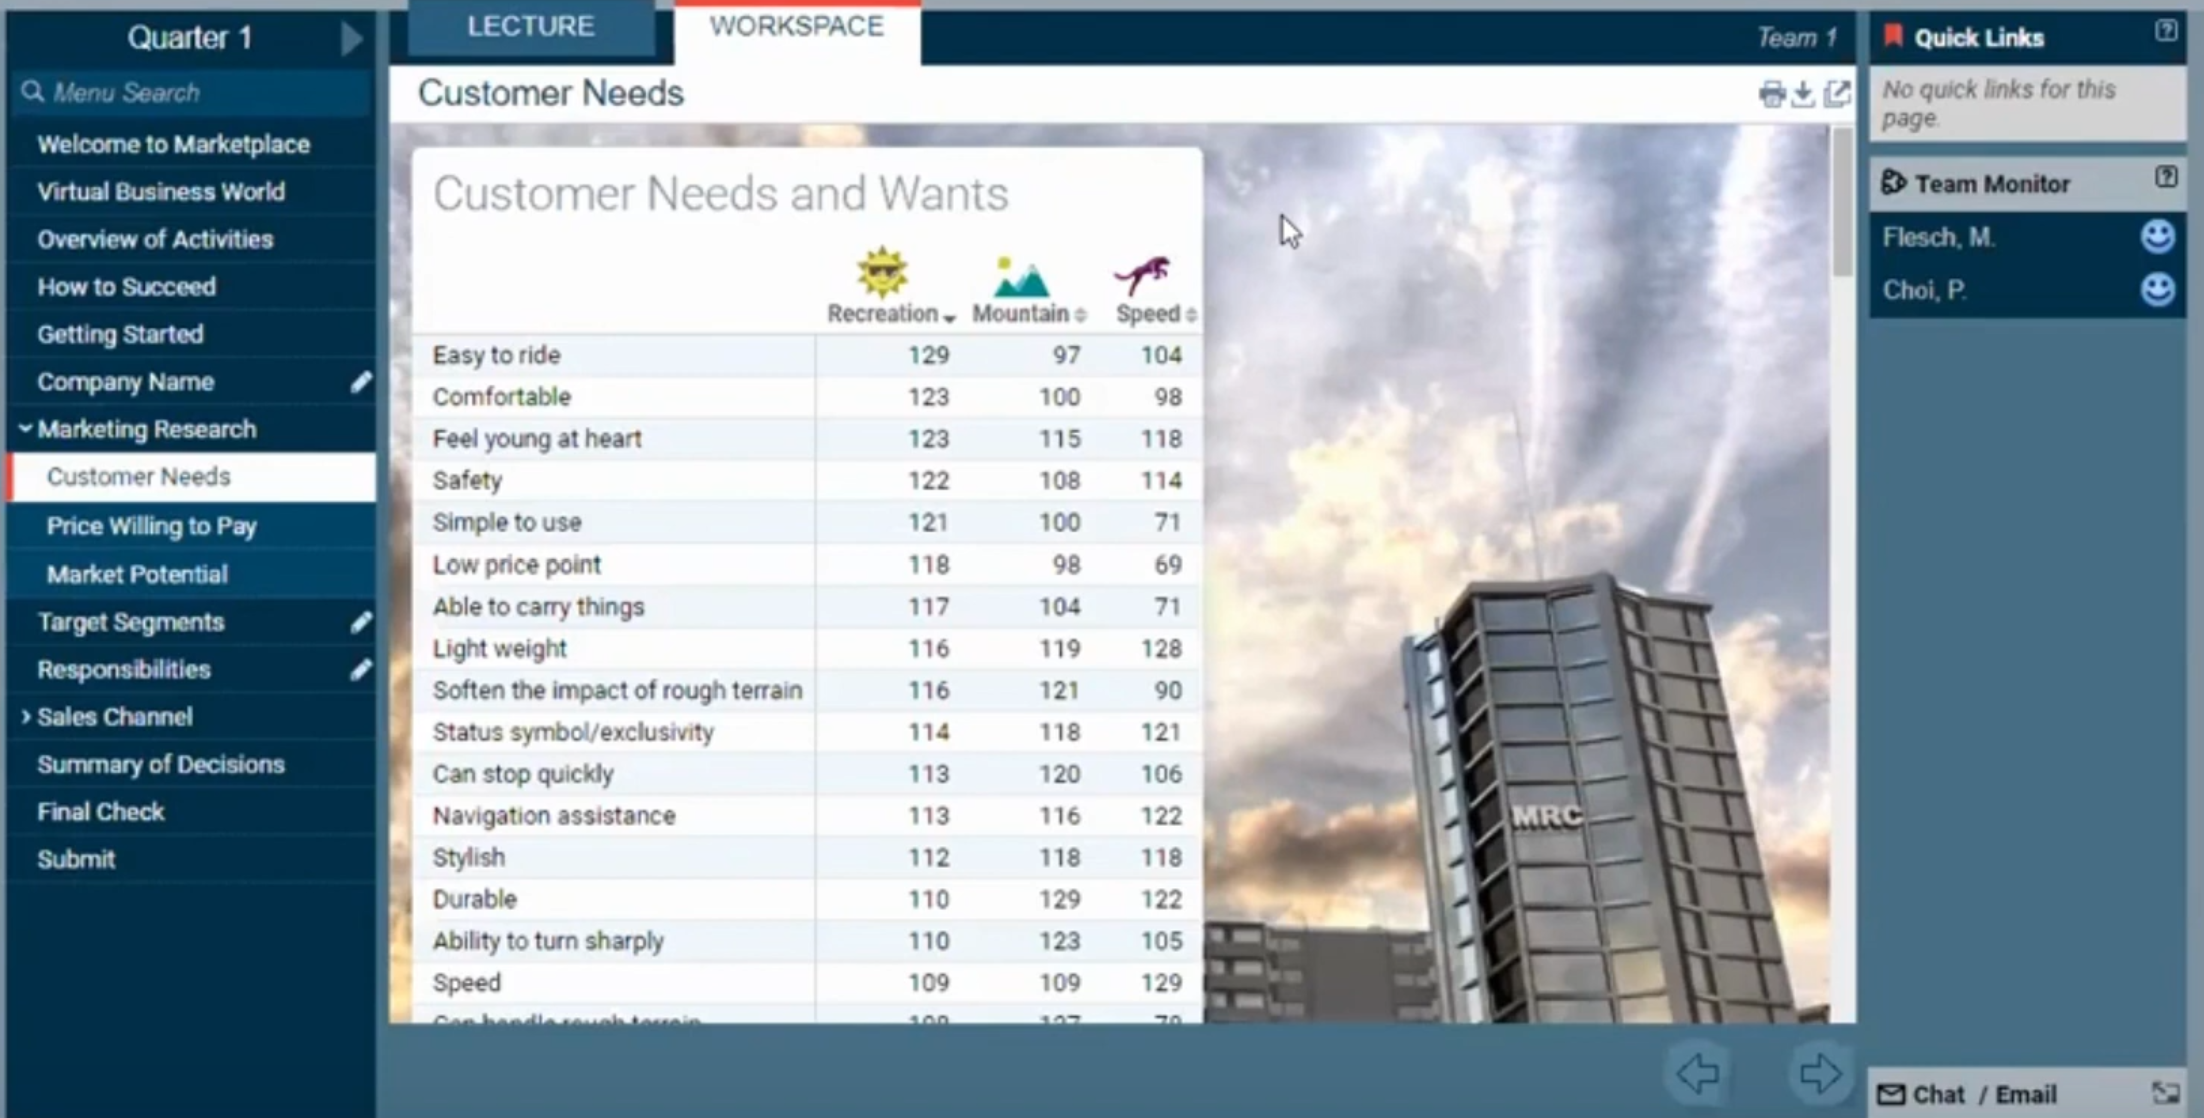
\includegraphics[max width=\textwidth]{./img/marketplace1}
 \caption{Captura de ecrã da aplicação \textit{International Corporate Management}}
 \label{fig:marketplace1}
 \end{figure}

Nesta plataforma, cada grupo de alunos representa uma empresa que tem de atuar num mercado internacional, tomando decisões sobre o posicionamento de produto, investimento, preços, distribuição, entre outras opções. Essas decisões são processadas pela plataforma, que simula o comportamento do mercado com base num algoritmo interno. 

A evolução temporal da simulação é dada por \textit{quarters}, que representam uma semana simulada. No final de cada \textit{quarter}, os alunos recebem os dados com os resultados das decisões anteriores, o que obriga a uma análise comparativa constante entre períodos. É este ciclo (decidir, analisar, ajustar, repetir) que dá sentido à simulação e aproxima o exercício a uma situação real.

A simulação está dividida em secções, cada uma representando uma área distinta do negócio gerido pelos alunos. Estas secções agrupam métricas, decisões ou outras informações relacionadas com aspetos específicos da empresa simulada, como por exemplo a procura por segmento, o desempenho financeiro, a perceção da marca ou a eficácia da força de vendas.

Cada secção representa também uma área onde os alunos têm de tomar decisões. As decisões variam consoante o tipo de secção, como por exemplo, na secção \textit{Customer Needs}, os alunos devem decidir que segmentos pretendem servir e com que marcas. Estas decisões são submetidas em cada ronda, influenciando os resultados seguintes, que por sua vez geram novos dados para análise.

A plataforma \textit{Marketplace Simulations – International Corporate Management} permite exportar os dados de cada secção em ficheiros Excel, sendo que cada ficheiro (ou folha dentro de um ficheiro) está associado a uma destas áreas. Exemplos comuns de secções incluem: \textit{Customer Needs}, \textit{Segment Demand}, \textit{Balanced Scorecard}, \textit{Sales Force Report}, entre outras.


Para a análise, os alunos têm à disposição os dados, na plataforma, nas várias secções disponiveis que na sua maioria são apresentados em tabelas, o que faz com que os alunos saltem entre secções, ou tenham de fazer gráficos à mão ou em último caso, extrair a informação da plataforma, não sendo então prático analisar a informação só pela plataforma de simulação.

\subsection{\textit{Pipelines Extract, Transform Load}}
\label{ch:etl}

Uma \textit{pipeline} \gls{etl} é um processo utilizado em sistemas de tratamento e integração de dados, com o objetivo de mover dados de uma ou mais fontes para um destino, geralmente uma base de dados ou um sistema de análise. O nome \gls{etl} representa as três etapas principais:

\begin{itemize}
  \item \textit{Extract} (Extrair): consiste em recolher os dados de múltiplas fontes de informação, que podem incluir bases de dados relacionais, APIs externas, sensores, entre outros. Esta fase preocupa-se com a capacidade de ler dados e de confirmar que são possiveis de extrair.
  
  \item \textit{Transform} (Transformar): nesta etapa os dados extraídos são processados e convertidos num formato mais adequado ao destino. Isso pode incluir tarefas como limpeza de dados (remoção de valores nulos ou duplicados), normalização, agregações, mudanças de tipo, ou cálculos. É nesta fase em que se garante a consistência da informação.

  \item \textit{Load} (Carregar): por fim, os dados transformados são inseridos na aplicação de destino, normalmente um \textit{data warehouse},  O carregamento é feito dependendo dos requisitos da aplicação de destino

\end{itemize}

As \textit{pipelines} \gls{etl} são muito utilizadas em contextos onde há necessidade de consolidar dados de várias origens, permitindo análises mais completas. São fundamentais em áreas como \textit{business intelligence}, ciência de dados e integração de sistemas.


\subsection{Padrão Cliente-Servidor}

O projeto desenvolvido segue uma arquitetura de aplicações cliente-servidor, dividida em duas grandes camadas: \textit{backend} e \textit{frontend}.

\textbf{\textit{Backend}}

O \textit{backend} corresponde a “parte invisível” da aplicação, ou seja, tudo o que acontece do lado do servidor. É a camada responsável por tratar os dados, executar a lógica de negócio e responder aos pedidos efetuados pelos utilizadores. No contexto específico deste projeto, o \textit{backend} é responsável por:

\begin{itemize}
    \item carregamento de ficheiros;
    \item processamento e normalização dos dados;
    \item autenticação e gestão de sessões;
    \item disponibilização de uma \gls{api} para o \textit{frontend} que permita acesso aos dados.
\end{itemize}

\textbf{Frontend}

O \textit{frontend} corresponde à ``parte visível'' da aplicação, ou seja, aquilo que o utilizador vê e com que interage diretamente no \textit{browser}. É a camada responsável por apresentar a informação de forma clara e permitir a interação com as funcionalidades disponibilizadas pela aplicação. No contexto deste projeto, o \textit{frontend} é responsável por:
\begin{itemize}
    \item os formulários, utilizados por exemplo para autenticação, criação de trimestres e envio de ficheiros;
    \item os gráficos, que permitem visualizar de forma interativa os dados transformados e filtrados pelo \textit{backend};
    \item e outros elementos visuais criados a partir dos dados processados, como tabelas, seletores de trimestre, mensagens de erro ou confirmação, entre outros.
\end{itemize}

Esta separação entre \textit{backend} e \textit{frontend} facilita a manutenção da aplicação e permite que ambas as partes evoluam de forma independente, podendo até ser substituídas sem necessidade de reescrever a aplicação completo. As tecnologias utilizadas para o desenvolvimento serão descritas no capítulo \ref{sec:tec}.

\subsection{Tipos de gráficos}

Durante a análise efetuamos foram estudados diferentes tipos de visualizações que podiam ser aplicadas, de acordo com os dados que tinhamos disponíveis. Cada tipo de visualização foi escolhido com base na sua capacidade de representar visualmente os dados e a sua facilidade de interpretação. 

Durante o desenvolvimento do projeto, foram considerados vários tipos de visualizações gráficas. Importa salientar que as imagens que acompanham esta secção foram retiradas diretamente da aplicação desenvolvida, já tendo em conta as limitações e as transformações realizadas nos dados. Estas transformações são discutidas mais a fundo no capítulo da análise inicial (ver capítulo \ref{sec:analiseInicial}).

\textbf{Gráfico de Barras (\textit{Bar Chart}):}

Este tipo de visualização foi utilizado para comparar valores entre diferentes categorias, como marcas, cidades ou segmentos de mercado. A disposição visual das barras permite uma leitura rápida das diferenças de desempenho entre categorias, sendo útil para dados que não são temporais. Foi também utilizado a variante barras agrupadas, dependendo se havia necessidade de comparar valores entre categorias.


\begin{figure}[H]
\centering
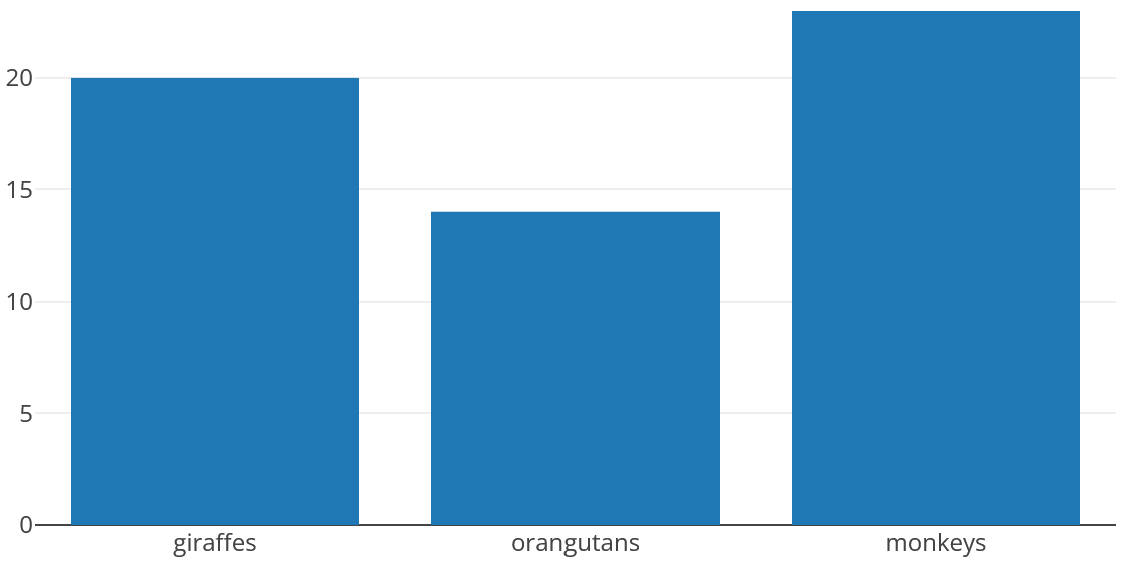
\includegraphics[max width=10cm]{./img/barras1}
\caption{Exemplo de gráfico de barras}
\end{figure}

\begin{figure}[H]
\centering
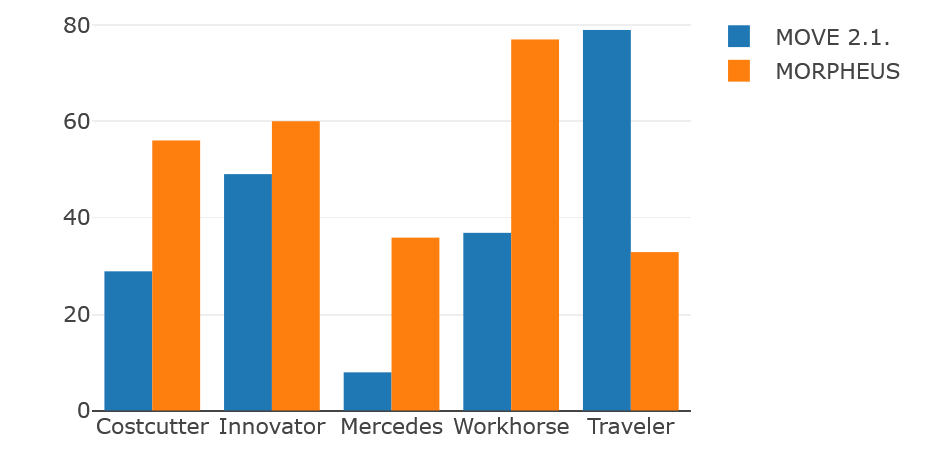
\includegraphics[max width=10cm]{./img/agrupada}
\caption{Exemplo de gráfico de barras agrupadas}
\end{figure}

\textbf{Gráfico de Sectores (\textit{Pie Chart}):}  

Utilizado para representar distribuições percentuais, como partições de dados por segmento. Este tipo é de gráfico é intuitivo para visualizar como uma totalidade se divide entre diferentes partes, sendo apropriado para dados onde se pretendia mostrar proporções relativas (como por exemplo dados categorizados por segmentos)

\begin{figure}[H]
    \centering
    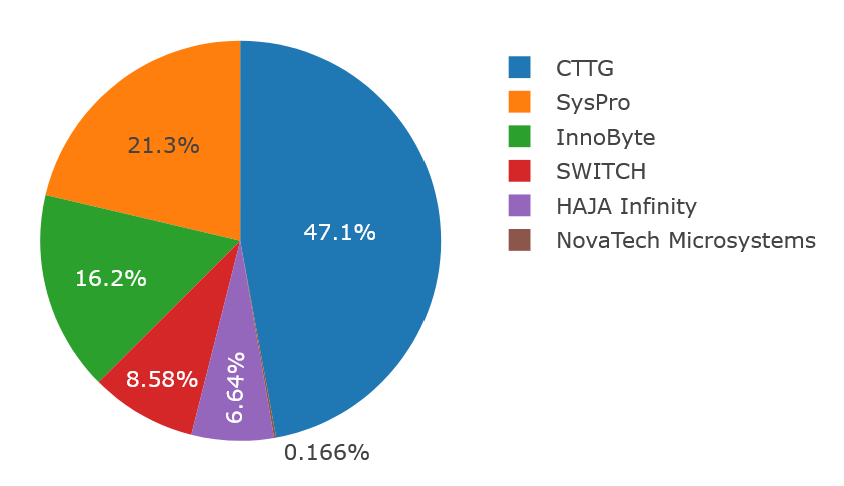
\includegraphics[max width=10cm]{./img/pie}
    \caption{Exemplo de gráfico de sectores}
\end{figure}

\textbf{Gráfico Financeiro (\textit{Waterfall Chart}):}  

Utilizado especificamente para representar balanços financeiros, como valores acumulados de receitas e despesas. Permite também visualizar como diferentes contribuições individuais afetam um valor final, facilitando a análise de ganhos e perdas.

\begin{figure}[H]
    \centering
    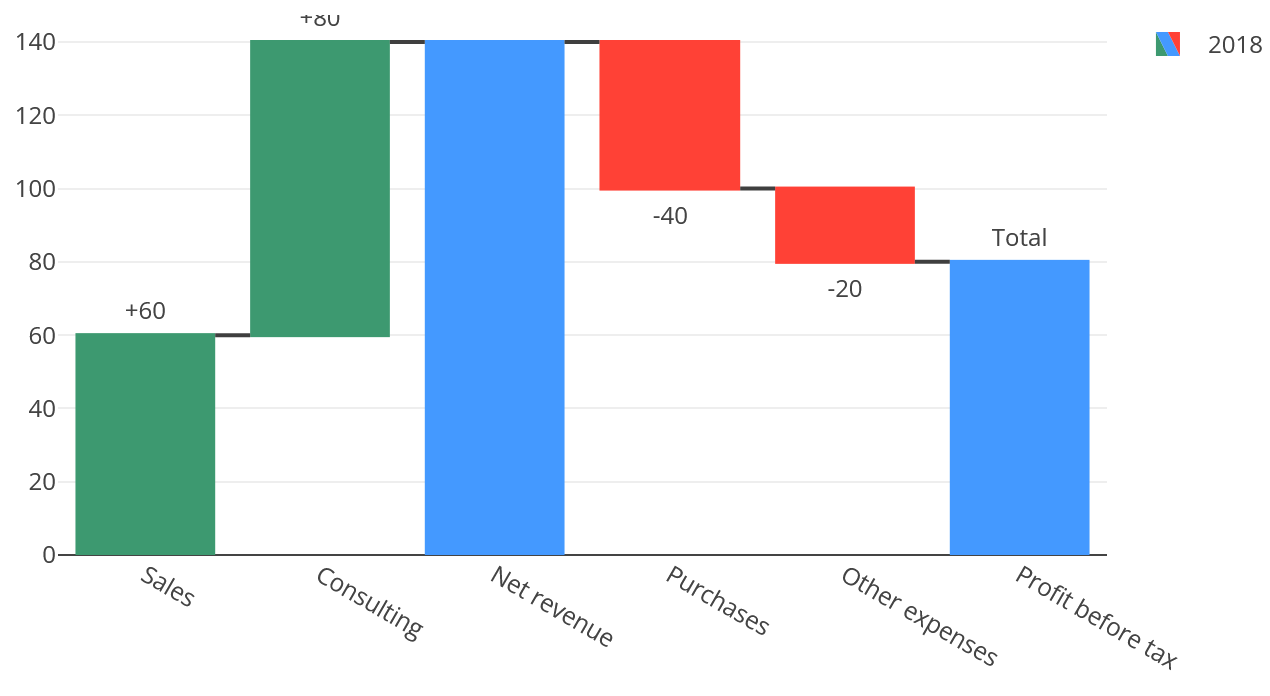
\includegraphics[max width=10cm]{./img/waterfall}
    \caption{Exemplo de gráfico financeiro}
\end{figure}

\textbf{Diagrama de Quartis (\textit{Box Plot}):}

Os diagramas de quartis foram utilizados para representar dados que eram distribuições com minimos e máximos, permitindo visualizar de forma prática a mediana, os quartis e valores extremos.  A interpretação deste tipo de visualização exige um conhecimento prévio de conceitos estatísticos como mediana e quartis, o que pode dificultar a leitura, mas que simplifica a representação dos dados.

\begin{figure}[H]
    \centering
    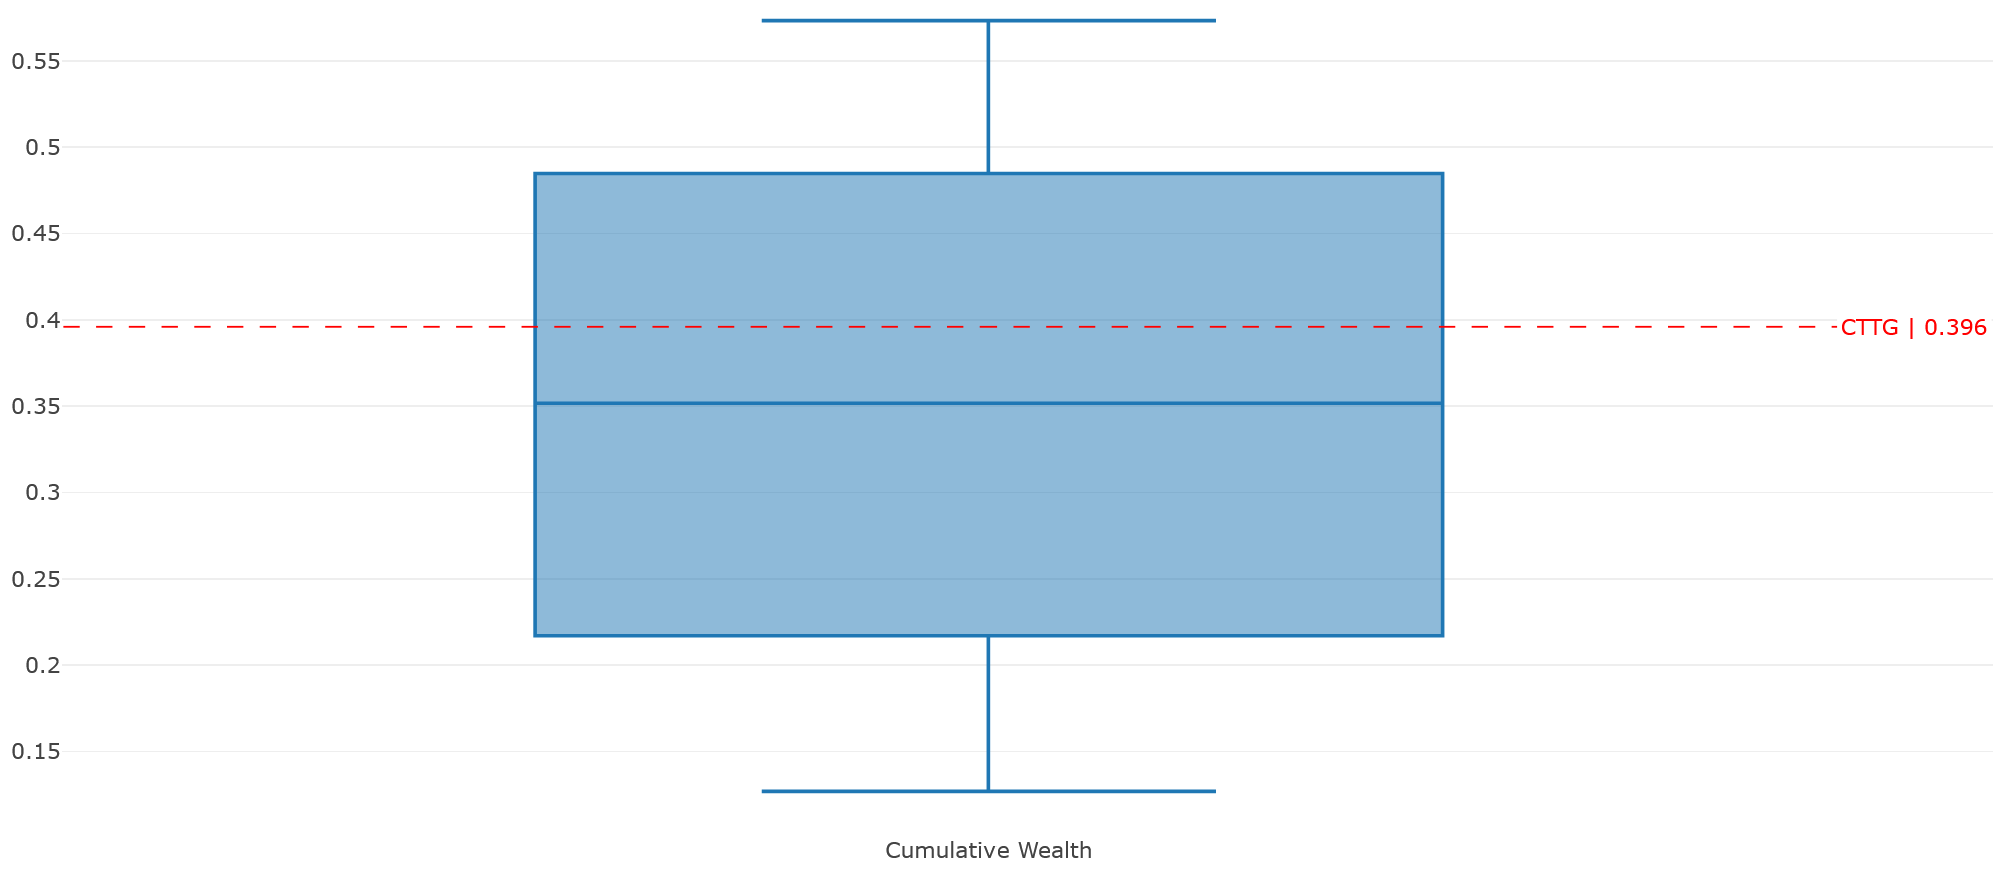
\includegraphics[max width=10cm]{./img/box}
    \caption{Exemplo de diagrama de quartis}
\end{figure}

\textbf{Diagrama de Sankey (\textit{Sankey Diagram}):}

Os diagramas de Sankey são utilizados para representar fluxos entre diferentes categorias, sublinhando a quantidade transferida de uma categoria para outra. Cada fluxo é representado por uma linha cuja largura é proporcional à quantidade movida, permitindo uma visualização intuitiva da importancia dos fluxos. Para evitar representações complexas, decidimos apenas recorrer a este tipo apenas quando os dados não poderiam ser representados de outra forma, ou tratados de forma a simplificar a representação.

\begin{figure}[H]
    \centering
    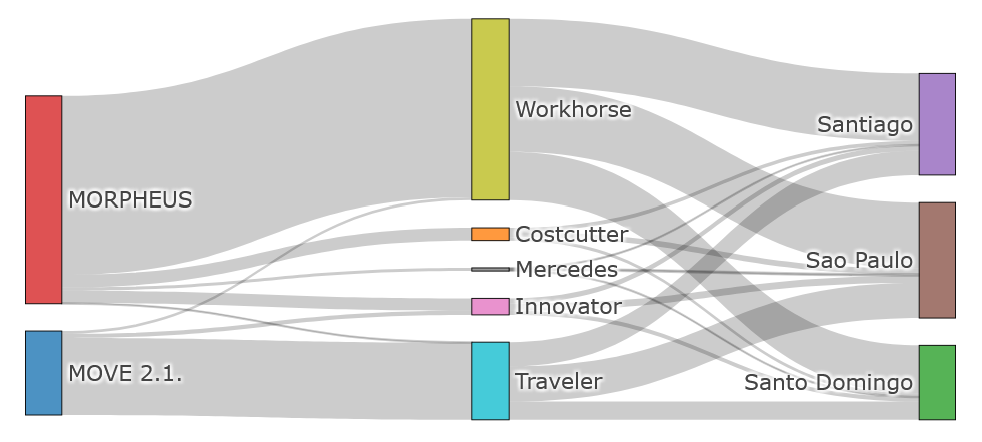
\includegraphics[max width=10cm]{./img/skankey}
    \caption{Exemplo de gráfico de Sankey}
\end{figure}

Outros tipos de gráficos relevantes para o projeto, mas que não foram utilizados são:

\textbf{Gráfico de Linhas (\textit{Line Chart}):}  

Escolhido para representar séries temporais, como a evolução de uma variável ao longo do tempo. As linhas permitem identificar tendências e variações. No projeto, não tivemos necessidade de usar este tipo uma vez que nenhum dos dados recebidos era relativos a séries temporais, pelo que a sua utilização não era intuitiva para os utilizadores nem resultava numa visualização que fizesse sentido para os dados recebidos.

\textbf{Gráfico de Radar (\textit{Radar Chart}):}  

Utilizado para comparar múltiplas variáveis em relação a um valor comum, como no caso da avaliação de diferentes necessidades dos clientes em simultâneo. Este tipo de gráfico permite identificar rapidamente pontos fortes e fracos em várias dimensões de análise. Apesar destas vantagens, nos dados que recebemos não conseguimos identificar utilizações onde este tipo de gráfico beneficiasse os utilizadores finais.

\textbf{Gráfico de Dispersão (\textit{Scatter Plot}):}

Os gráficos de dispersão foram considerados para representar relações entre duas variáveis. Cada ponto no gráfico representa uma observação individual, permitindo identificar padrões de correlação (positiva, negativa ou inexistente) entre variáveis. No nosso caso, consideramos utilizar um tipo especifico de gráfico de dispersão (gráfico de dispersão num mapa) mas a leitura tornou-se confusa, uma vez que era pouco legivel para alunos, e não considerava localizações ficticias, fazendo com que a leitura fosse difícil, como pode ser visto na figura  \label{fig:scatter-map}, que é um gráfico do tipo \textit{scatter map} feito com dados importados de uma folha de cálculo, em que os pontos estão muito dispersos, num mapa que contem várias referencias a cidades, e sem representação do valor numérico associado (aparece um ponto azul).

\begin{figure}[H]
    \centering
    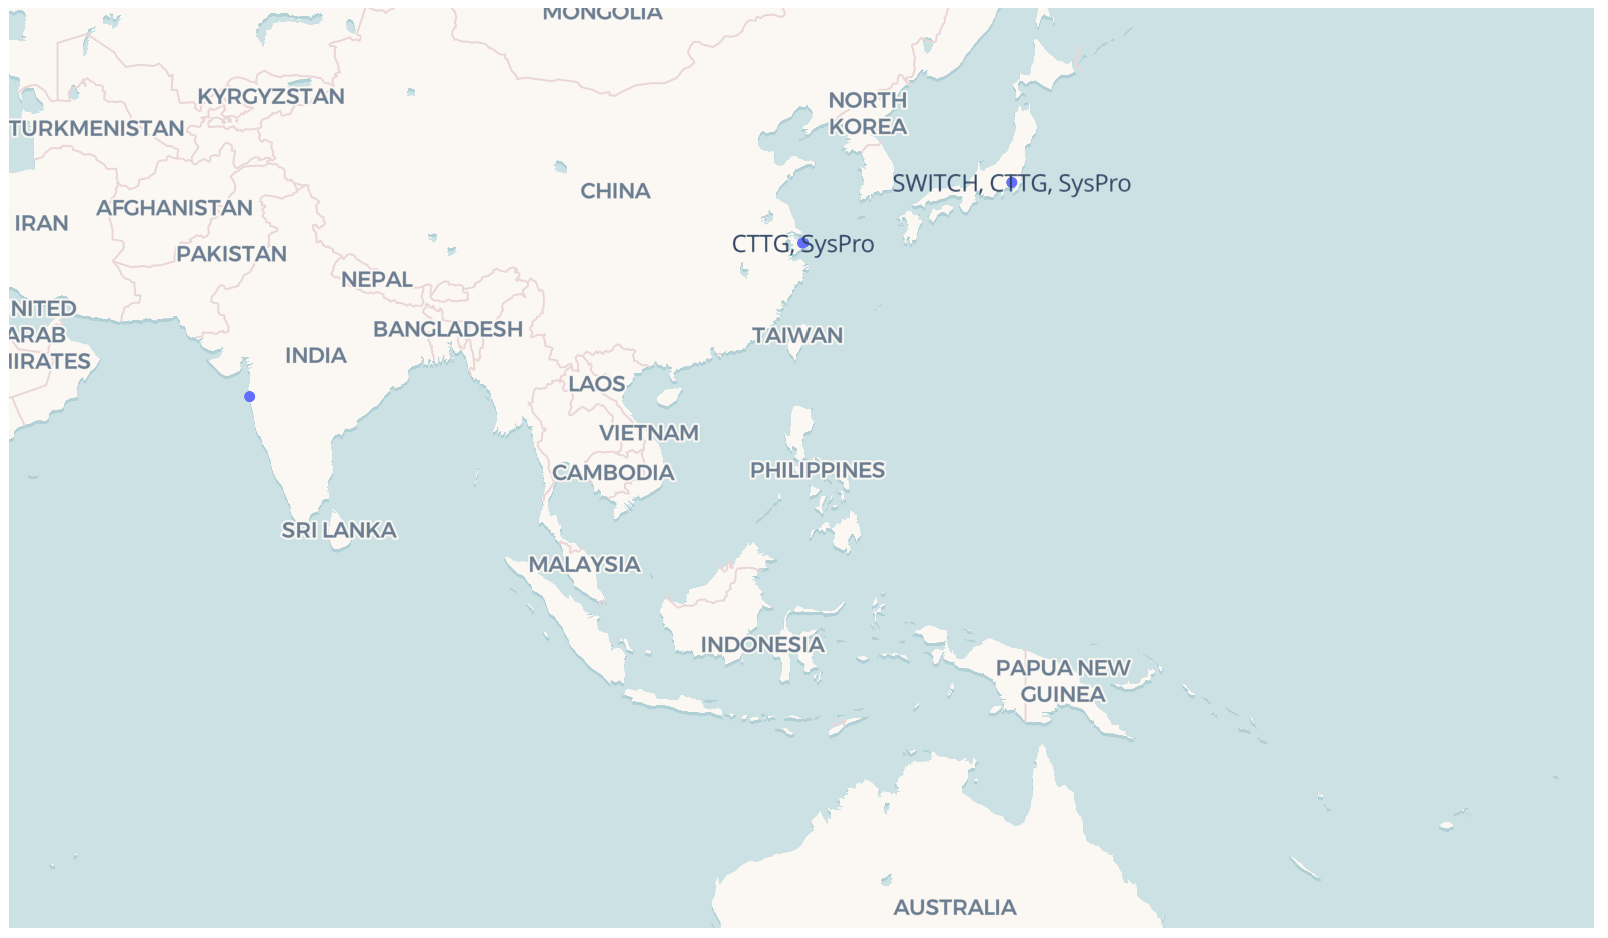
\includegraphics[max width=10cm]{./img/scatter_map}
    \caption{Exemplo de gráfico de dispersão num mapa}
    \label{fig:scatter-map}
\end{figure}
\noindent

A imagem acima não apresenta uma boa leitura, pelo que optámos por não incluir este gráfico nas nossas representações.

\end{itemize}

A escolha dos tipos de gráficos teve como objetivo manter a clareza e facilidade da informação e permitir diferentes leituras sobre os dados extraídos. Cada gráfico foi pensado para às características das categorias disponíveis, considerando tanto a o formato dos dados (quantitativa ou categórica) como o objetivo da análise (comparação, distribuição, evolução ou composição).

%%________________________________________________________________________
\section{Abordagem}
\label{sec:abordagem}
%%________________________________________________________________________

O projeto proposto pretende então ajudar nesse sentido, de conseguir transformar dados desta plataforma em algo mais fácil e rápido de analisar. Tendo o contexto da plataforma, iremos então descrever duas abordagens que considerámos.

\subsection{\textit{Web \textit{scraping}}}

A primeira abordagem que consideramos foi a hipótese de automatizar a extração dos dados diretamente da plataforma do Marketplace Simulations, através de técnicas de \textit{web} \textit{scraping}. A ideia parecia interessante numa fase inicial, já que permitiria reduzir a dependência do utilizador no processo de exportação  dos dados. No entanto, rapidamente percebemos que esta abordagem trazia vários desafios que, na prática, a tornavam pouco viável, ou mesmo arriscada.

Primeiro, cada conta na plataforma está associada a um grupo de alunos, ou seja, é uma conta ativa e única, usada diretamente durante a simulação. Isto significa que qualquer processo automático que iniciasse sessão, mesmo que fosse só para leitura, poderia de forma acidental interagir com a interface e acabar por alterar alguma opção, o que poderia comprometer a avaliação dos alunos porque podia afetar a sua avaliação final. Além disso, como o acesso à plataforma é feito por licenças pagas, não existe qualquer possibilidade de criar uma conta de serviço ou utilizador apenas para leitura. Ou seja, qualquer tentativa de \textit{web} \textit{scraping} teria de reutilizar credenciais reais, o que levanta não só questões de segurança, mas também (possivelmente) legais, uma vez que a plataforma pode não permitir o \textit{web} \textit{scraping}.

Outro fator que influenciou a nossa decisão foi o próprio risco técnico do \textit{web} \textit{scraping} uma vez que plataformas deste tipo estão muitas vezes protegidas com mecanismos contra automação (como por exemplo ecrãs CAPTCHA), e não conhecendo em detalhe a aplicação, poderíamos facilmente encontrar esse tipo de proteções, que são difíceis de automatizar.

Pelos motivos acima, optámos por não seguir esta abordagem. Em vez disso, definimos como parte da utilização da nossa aplicação que os próprios alunos devem exportar dados a partir da plataforma de simulação e carregar para a nossa aplicação. Esta solução, embora mais manual, garante segurança, respeita a integridade das contas dos utilizadores, e evita problemas legais ou técnicos com a aplicação de simulação.

\subsection{Exportação e carregamento manual de ficheiros}

A abordagem que acabamos por usar foi os alunos exportam manualmente os dados diretamente da plataforma de simulação e carregarem esses ficheiros na nossa plataforma. A partir daí, a aplicação processa e normaliza os dados recebidos, e mostra gráficos com base nesses dados. Esta abordagem, apesar de requerer uma ação manual do lado do utilizador, é mais segura que a alternativa de \textit{web} \textit{web} \textit{scraping}, pelos os motivos apresentados acima. Deste modo, garantimos um equilíbrio entre usabilidade, segurança e fiabilidade da aplicação. Acabamos então por criar um \gls{sad} (\cf, capítulo \ref{sec:sad}) que permita os estudantes tomarem melhores decisões.

Com esse objetivo, procurámos que a nossa aplicação refletisse a estrutura da própria simulação. Como tal, os dados são organizados por \textit{quarters}, como acontece na plataforma de simulação e permitir o carregamento dos dados exportados. Estes ficheiros são depois processados o que nos permite trabalhar com dados mais consistentes. 

Esta estrutura base implica a existência de três entidades principais na nossa aplicação (que iremos descrever nos capítulos seguintes) e cuja interação define  o funcionamento da aplicação.

\subsubsection{\textit{Quarters}}

Os \textit{quarters} funcionam como \textit{buckets} para organizar os ficheiros carregados pelos utilizadores. Cada utilizador pode criar múltiplos \textit{quarters}, identificados de forma única por um número. O propósito em incluir este conceito é para que a aplicação consiga associar os dados extraidos dos ficheiros carregados ao \textit{quarter} correspondente sem depender de manipulações do nome do ficheiro carregado, e desde modo assegurar que a plataforma consegue identificar corretamente os \textit{quarters}. 

A desvantagem é que requer \textit{input} do utilizador para que seja criado ou atribuído o \textit{quarter} correto. De modo a facilitar a criação de \textit{quarters}, tentamos que experiência de utilização fosse centrada no carregamento de ficheiros, limitando os \textit{quarters} a um campo obrigatório no formulário de carregamento auto-preenchido, ou seja, tornando implicita a criação de \textit{quarters} no momento de carregamento de ficheiros.

\subsubsection{Ficheiros}

Os ficheiros são inicialmente carregados no formato \gls{xlsx} (que é o formato que a plataforma de simulação exporta), contendo uma ou várias folhas de cálculo. Cada folha é tratada como uma fonte de dados individual e é de onde são extraidos os dados. O ficheiro \gls{xlsx} é guardado como referência, mas não é diretamente utilizado para visualização, ficando apenas como artefacto interno da aplicação. O modelo proposto não prevê que uma folha de cálculo origine multiplos gráficos.

O processamento que é aplicado é uma \textit{pipeline} de transformação de dados (conhecido na industria como \gls{etl} (\cf, capítulo \ref{ch:etl})), que aplica regras para que os gráficos possam ser mostrados de forma consistente. Os dados resultantes desta transformação estão associados ao ficheiro \gls{xlsx} original, sendo até possivel voltar a processar ficheiros de forma a recriar informação (esta funcionalidade não é disponibilizada aos utilizadores finais e não foi desenvolvida de forma explícita).

A plataforma garante que só existe uma versão ativa de cada ficheiro. Caso o utilizador carregue novamente um ficheiro com o mesmo nome, o anterior será marcado como não ativo, evitando duplicações e garantindo que os gráficos usam apenas dados mais recentes, e em caso de remoção, garante que conseguimos reverter para a versão anterior.

\subsubsection{\textit{Pipeline} de Transformação de Dados}

Para conseguirmos então garantir uma experiência de utilização consistente, desenvolvemos uma \textit{pipeline} transformação de dados, semelhante a uma \textit{pipeline} \gls{etl} (\cf, capítulo \ref{ch:etl}), ainda que neste projeto tenha sido desenvolvido com uma escala mais pequena, e com recurso a bibliotecas de processamento de dados. 

O objetivo é garantir que os ficheiros carregados, que muitas vezes contêm nomes de colunas inconsistentes, quebras de linha, espaços em excesso ou colunas irrelevantes, sejam adaptados para serem visualizados, e que o processamento seja deterministico.

Como podemos receber muitos ficheiros, a variabilidade entre os dados recebidos é muito alta, pelo que alguns dados passam por mais do que uma fase de transformação. Esta decisão foi tomada com base numa análise manual, em que identificámos possíveis fontes de dados que precisam de mais do que uma fase de transformação. As várias fases de transformação alteram os dados de modo a facilitar a representação visual dos mesmos e é um passo essencial no projeto, porque garante que a aplicação trabalha com formatos e regras conhecidas, e remove a variabilidade dos ficheiros importados. Para proteger a aplicação, decidimos apenas mostrar os dados que foram extraidos de ficheiros conhecidos, de modo a garantir a consistencia dos dados mostrados.

As fases de transformação irão ser descritas em mais detalhe nos capítulos seguintes, uma vez que a implementação destas pipeline estão relacionadas à tecnologia escolhida, mas o desenvolvimento desta \textit{pipeline} é um fator diferenciador deste projeto, uma vez que tem de lidar com dados que não estão estruturados de forma a facilitar representações visuais. 

\subsubsection{Utilizadores}

A plataforma foi projetada para funcionar com utilizadores. Cada utilizador tem a sua conta, e pode criar \textit{quarters}, carregar ou alterar ficheiros, e ver aos gráficos gerados a partir desses ficheiros.

Apesar da plataforma não suportar explicitamente equipas ou grupos, assume-se que alunos do mesmo grupo podem carregar ficheiros semelhantes, mas a aplicação trata-os como ficheiros diferentes. Assim, evita-se a complexidade adicional de gerir permissões ou partilha de dados entre contas. 

Também se assume que as contas podem ser criadas ao nível do grupo, pelo que para a plataforma, é indiferente se a conta é individual ou partilhada entre membros desse grupo.

Cada utilizador tem acesso apenas aos seus próprios dados, garantindo o isolamento da informação. Esta separação é feita a nível da base de dados, através da associação de cada entidade ao utilizador que criou.

No futuro, pode ser considerada a funcionalidade de desativação automática de contas (por exemplo, após o final do semestre), mas para já o modelo é simples, conta individual, dados isolados, e controlo completo sobre os próprios \textit{uploads}.

No próximo capitulo iremos então descrever as escolhas tomadas de forma a concretizar este modelo.

\section{Arquitetura e Tecnologias Adotadas}
\label{sec:tec}

\begin{figure}[h]
\centering
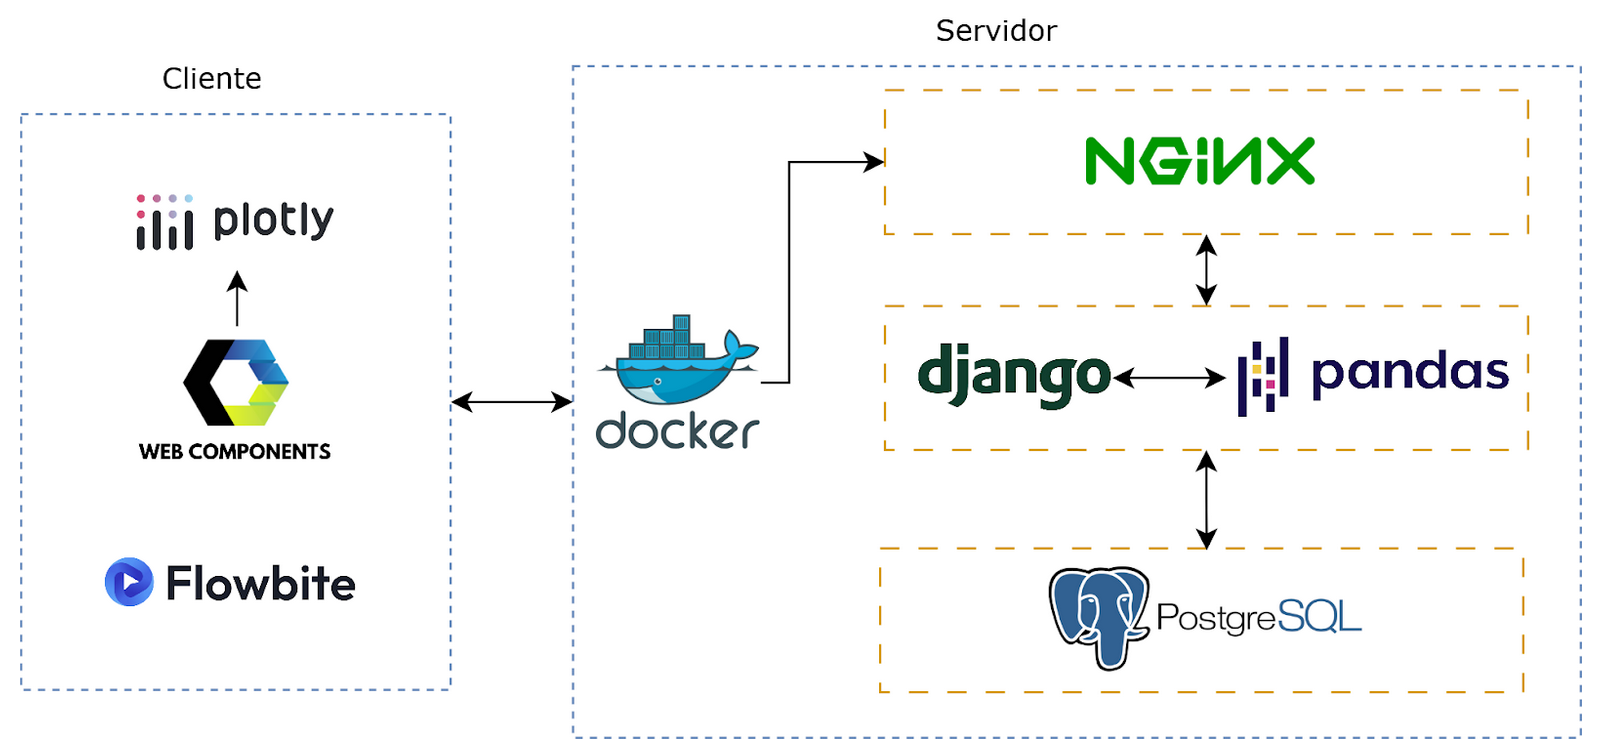
\includegraphics[max width=\textwidth]{./img/arch}
\caption{Arquitetura da aplicação}
\label{fig:arquitectura}
\end{figure}

A arquitetura final da aplicação pode ser observada na Figura~\ref{fig:arquitectura}. Esta segue o modelo cliente-servidor, onde os utilizadores interagem com a aplicação através de um \textit{browser}. A definição da arquitetura, a seleção das tecnologias e a organização dos dados foram guiadas por critérios de fiabilidade, simplicidade de manutenção e possibilidade de evolução futura.  Nas seguintes secções especificamos que tecnologias escolhemos e que funções desempenham na aplicação.

\subsection{Django}

Para o desenvolvimento do \textit{backend} da aplicação, optámos por usar a \textit{framework} \textit{Django}. A escolha deveu-se ao facto de o \textit{Django} ser uma \textit{framework} muito usada, com uma arquitetura conhecida e uma comunidade grande.

Uma das principais vantagens do \textit{Django} é o facto de seguir o padrão de arquitetura \gls{mvc}, o que facilita bastante a organização da aplicação e a separação de responsabilidades. No entanto, o \textit{Django} utiliza uma variante própria deste padrão, conhecida como \gls{mtv} onde:

\begin{itemize}
    \item o \textit{Model} representa a camada de dados e corresponde ao modelo do domínio;

    \item o \textit{Template} representa a camada de apresentação (interface com o utilizador);

    \item a \textit{View}, em \textit{Django}, atua como o controlador que processa a lógica da aplicação e interage com os modelos e os templates.
\end{itemize}

Apesar da diferença de nomes, esta arquitetura cumpre os mesmos princípios do padrão \gls{mvc} tradicional \cite{fitzgerald2007web,djangodocs}, promovendo uma clara separação de preocupações, o que facilita o desenvolvimento, testes e manutenção da aplicação.

Para além disso, o \textit{Django} oferece um \gls{orm} integrado, que permite interagir com bases de dados de forma mais intuitiva, sem necessidade de escrever \gls{sql} manualmente. Este ORM permite mapear modelos Python em tabelas relacionais e suporta operações como filtros, agregações e relações entre tabelas \cite{djangodocs}, ao mesmo tempo que previne falhas comuns de segurança como \textit{SQL injection} através do uso de consultas parametrizadas \cite{kumar2016security}.

Outra vantagem é a gestão de utilizadores, permissões e sessões já estar incluída de forma nativa no \textit{framework}, facilitando a autenticação, autorização e persistência de sessões de utilizador \cite{djangodocs}. Isto permite ao programador focar-se no desenvolvimento das funcionalidades específicas da aplicação sem ter de construir esse suporte de raiz.

Outro fator que consideramos positivo foi a integração com outras bibliotecas Python, como o \textit{Pandas}, que usamos para o processamento de dados. Esta compatibilidade torna o desenvolvimento mais rápido e flexível, reduzindo o esforço necessário para ligar diferentes tecnologias. O ecossistema Python é particularmente forte no tratamento de dados, e o Django, sendo escrito em Python, tira partido disso de forma direta \cite{vanrossum2001python}.

Em alternativa, podiamos ter escolhido bibliotecas como \textit{Flask} ou \textit{FastAPI}. Apesar de \textit{FastAPI} ser mais recente e mais rápido para \texit{API} \gls{rest} \cite{tiangolo2018fastapi}, o nossa aplicação, focado na transformação de dados e visualização, não necessitava de uma abordagem completamente assíncrona e não funciona totalmente com \texit{API}s \gls{rest}. Já o \textit{Flask}, apesar de ser mais leve, implicaria uma maior responsabilidade na definição de toda a arquitetura e gestão de utilizadores, e que aumentava a complexidade do projeto \cite{grinberg2018flask}.

Relativamente a outras opções como \textit{WordPress}, excluímos essa hipótese. O \textit{WordPress}, ainda que muito prática de servir de suporte para sites de conteúdo como blogues ou sites de noticias, não é adequado para projetos que exigem controlo total sobre a estrutura dos dados, processamento no \textit{backend} e não integra bem com as outras tecnologias escolhidas.

\subsection{Pandas}

Para o processamento de dados, a biblioteca que decidimos usar foi o \textit{Pandas}. Esta escolha foi motivada pelo facto de ser muito utilizada em projetos de engenharia de dados, e por ser escrita em \texit{Python}.

O \textit{Pandas} permite ler e transformar ficheiros Excel com facilidade. A sua sintaxe e as funcionalidades para operações como normalização, filtragem, agrupamento ou ordenação tornaram-na adequada para as tarefas necessárias neste projeto.  Outra vantagem mais é a capacidade de converter os dados diretamente para formatos como \gls{json}, o que facilitou a sua integração com o resto da aplicação.

Apesar destas vantagens, o \textit{Pandas} não é a melhor opção se considerarmos \textit{datasets} muito grandes, uma vez que funciona inteiramente em memória. Em contextos com maiores volumes de dados, poderiam ser consideradas bibliotecas como \textit{Dask} ou \textit{Polars} por terem capacidades de paralelismo para lidar com um maior conjunto de dados (acabam por ser mais adequadas para \textit{BigData}). No entanto, para os objetivos e escala deste projeto, o \textit{Pandas} é a escolha mais equilibrada considerando o scope do projeto que desenvolvemos.

\subsection{Plotly}

Para mostrar os gráficos da aplicação, optámos por utilizar o \textit{Plotly}, que é uma biblioteca  que permite criar visualizações, e que está disponivel em várias linguagens como \texit{Python} e \texit{Javascript}. Esta escolha foi motivada pelo facto de o \textit{Plotly} suportar suportar uma \texit{API} declarativa, o que torna mais prática a integração com o \textit{frontend} e \textit{backend}, porque assim a configuração dos gráficos pode ser retornada pelo servidor, permitindo uma configuração mais estável e garantindo que todos os utilizadores vêm o mesmo tipo de gráfico. Internamente, o \textit{Plotly} utiliza uma outra biblioteca, \textit{D3.js}, que é uma biblioteca com capacidade de criar gráficos personalizados.

Além disso, a biblioteca oferece suporte a uma grande variedade de gráficos, desde os mais comuns (barras, linhas, circulares) até formatos mais especializados (como gráficos de cascata ou mapas de calor), o que foi importante para explorar os vários tipos de visualização que estavamos a considerar usar. Em comparação, bibliotecas como \textit{Chart.js}, embora sejam mais leves, limitam-se a um conjunto reduzido de gráficos e oferecem menos controlo sobre detalhes de visualização. Por este motivo, \textit{Plotly} era a solução mais adequada para a flexibilidade e diversidade de visualizações que queriamos. Uma lista completa das diferencas pode ser consultada no (\cf, capítulo \ref{ch:charts}).

A versão \textit{Python} desta biblioteca foi também importante no desenvolvimento dos gráficos, uma vez que nos permitiu explorar os dados de forma independente da aplicação (fora da aplicação) de modo escolher que tipo de gráfico seria o mais adequado aos dados que estavamos a analisar e que transformações eram necessárias para obter os gráficos escolhidos. Este processo de exploração permitiu-nos perceber o que era possível fazer, e com a ajuda dos orientadores, definir estratégias alternativas para os conjuntos de informação que queríamos mostrar.

\subsection{\textit{WebComponents}}

No \textit{frontend}, decidimos utilizar \textit{WebComponents} \cite{webcomponents}, sem recorrer a \textit{frameworks} como \textit{React} ou \textit{Vue}. Esta decisão teve como base a necessidade de criar uma interface leve, e garantir que a aplicação reage aos \textit{inputs} do utilizador. 

Os \textit{WebComponents} \cite{webcomponents} são uma especificação nativa dos \textit{browsers}, que permite definir componentes reutilizáveis com encapsulamento de estilo e comportamento. Ao evitarmos dependências pesadas como o \textit{React}, conseguimos reduzir a complexidade técnica da aplicação, mantendo ao mesmo tempo a flexibilidade e capacidade de reutilização dos componentes desenvolvidos.

Apesar de \textit{React} ser uma framework muito utilizada para aplicações \textit{web},  com um ecossistema já muito maduro e uma comunidade grande, considerámos que para este projeto, a sua introdução seria um excesso em termos de dependências e complexidade. A alternativa escolhida proporcionou uma solução mais leve e mais fácil de manter. Outra razão que nos levou a esta escolha foi o facto do \textit{Django} já trazer consigo as funcionalidades de autenticação, pelo que se a aplicação \textit{web} fosse escrita totalmente em \textit{React}, teriamos de usar o \textit{Django} apenas como uma \gls{API} \gls{REST}, e utilizar métodos alternativos de autenticação como \textit{OAuth2}.

\subsection{\textit{PostgreSQL}}

Para a persistência de dados, utilizámos a aplicação de gestão de bases de dados \textit{PostgreSQL}, uma das soluções \textit{open-source} mais completas e robustas disponíveis atualmente. Inicialmente foi considerada a utilização de \textit{SQLite} por simplicidade durante o desenvolvimento, mas rapidamente a necessidade de maior escalabilidade e de suporte a funcionalidades como campos \gls{json}, levou à adoção do \textit{PostgreSQL}.

\textit{PostgreSQL} oferece um bom desempenho, suporte a operações complexas e é compatível com o \gls{orm} do \textit{Django}, o que permitiu tirar partido do modelo relacional sem abdicar da produtividade no desenvolvimento. Comparado com outras alternativas como \texit{MySQL}, o \textit{PostgreSQL} distingue-se pelo seu suporte avançado a tipos de dados (\gls{json}, \texit{arrays}, \textit{enums}), entre outras funcionalidades.


\subsection{Docker}

O \textit{Docker} foi utilizado neste projeto como solução de virtualização, tanto para desenvolvimento como para ambientes de produção. A principal vantagem da sua adoção prende-se com a criação de ambientes consistentes e isolados, garantindo que a aplicação corre da mesma forma em diferentes máquinas, sem conflitos de dependências ou configurações, e consistentemente em vários sistemas operativos. 

Existem vários \textit{runtimes} compativeis com \textit{Docker}, e devido ao modelo de negócio da empresa \textit{Docker} (que adotou um modelo pago), optámos por usar o \textit{Rancher} (uma aplicação com uma \gls{api} compatível com \textit{Docker}) para o desenvolvimento, e o \textit{Docker Engine} para ambientes de produção.

Durante o desenvolvimento, o \textit{Docker} facilitou a orquestração dos serviços necessários (a aplicação Django, a base de dados, e o servidor \gls{http} Nginx configurado como \textit{reverse proxy}), utilizando ficheiros \texttt{Dockerfile} e \texttt{docker-compose.yml}. Isto permitiu montar rapidamente o ambiente completo da aplicação, sem necessidade de instalações manuais por parte dos programadores.

Para produção, o \textit{Docker} permite recriar um ambiente de produção sempre com a mesma configuração e gerir os vários serviços que a aplicação utiliza, o que facilita o processo de \textit{deploy}, e escalabilidade futura. Esta abordagem garante que o código testado é exatamente o que será executado em produção, reduzindo erros e aumentando a estabilidade da aplicação.

O \textit{Docker} foi também utilizado durante o desenvolvimento deste relatório, porque permitiu-nos ter um ambiente \textit{LaTex} configurado com todas as extensões apenas com um único comando no terminal sem instalar aplicações.

\section{Outras ferramentas utilizadas}
\label{sec:tools}

Além das tecnologias centrais utilizadas no projeto, foi também fundamental a utilização de um conjunto de ferramentas de suporte que facilitaram o trabalho, a organização e o desenvolvimento do projeto. As principais ferramentas utilizadas foram:

\begin{itemize}
    \item \textbf{Git \cite{git} e Github \cite{github}}: Para assegurar o controlo de versões, foi utilizado a aplicação Git, em conjunto com a plataforma Github. Esta combinação permitiu não só manter um histórico  das alterações feitas, mas também garantir a colaboração e a integridade do desenvolvimento ao longo do tempo.

    \item \textbf{Notion \cite{notion}}: A gestão de tarefas e a organização de trabalho foram centralizadas na plataforma \textit{Notion}. Esta ferramenta é prática de fácil de usar, e para planear as tarefas, definir prioridades, acompanhar o progresso das diferentes fases do projeto. É também uma ferramenta muito fácil de usar, e que permite também tirar notas durante o desenvolvimento, que foram importantes para o desenvolvimento do relatório.

    \item \textbf{\gls{vscode}\cite{vscode}}: Como editor, foi utilizado o editor \gls{vscode}. Através da instalação de extensões, foi possível adaptar o \gls{vscode} às necessidades do projeto, melhorando a experiência de programação.
\end{itemize}

Estas ferramentas, utilizadas de forma consistente, desempenharam um papel importantes na execução do projeto, não só do ponto de vista técnico, mas também no que respeita à organização e planeamento do mesmo.

%%________________________________________________________________________
%% LEIM | PROJETO
%% 2022 / 2013 / 2012
%% Modelo para relatório
%% v04: alteração ADEETC para DEETC; outros ajustes
%% v03: correção de gralhas
%% v02: inclui anexo sobre utilização sistema controlo de versões
%% v01: original
%% PTS / MAR.2022 / MAI.2013 / 23.MAI.2012 (construído)
%%________________________________________________________________________




%%________________________________________________________________________
\chapter{Implementação do Modelo}
\label{ch:implementacaoDoModelo}
%%________________________________________________________________________

O desenvolvimento da aplicação assentou em fundamentos sólidos tanto ao nível tecnológico como ao nível das boas práticas de engenharia de software e tratamento de dados. A escolha da arquitetura, das tecnologias utilizadas e dos modelos de organização dos dados foi orientada por critérios de fiabilidade, modularidade, simplicidade de manutenção e escalabilidade.

\section{Arquitetura Tecnológica}
- Falar sobre \textit{stack} usada no projeto, alternativas e prós e contras

\section{Análise dos dados}
Nesta secção iremos descrever como analisamos a informação recebida da plataforma de simulação e as decisões tomadas sobre essa informação.

\subsection{Análise inicial da informação}
Após termos recebido os dados, fizemos uma primeira análise com o objetivo de perceber a informação recebida e os próximos passos a tomar. No total, recebemos 39 ficheiros \gls{xlsx} que foram exportados da plataforma, 

\subsection{Classificação da informação}

- Falar sobre como classificamos os 39 ficheiros Excell em "buckets" e cada bucket ficou com um "template" gráfico pré-determinado
- Falar sobre cada grupo, o que significa e o que todos os gráficos partilham em comum em cada grupo.

\subsection{Visualização escolhidas para os vários grupos}
- Falar sobre os vários

\section{Processamento dos dados}
- Iniciar o tema de processamento de informação, converter informação desconhecida para um formato normalizado.

\subsection{\textit{Pipeline} de transformação dos dados}
A primeira fase de normalização segue os seguintes passos:
\begin{itemize}
    \item Extrai o nome do gráfico a partir da primeira linha de cada folha.
    \item Usa a segunda linha como cabeçalhos e normaliza os nomes (ex: substitui espaços por \textit{underscores}, remove quebras de linha).
    \item Remove colunas irrelevantes com base numa lista de columnas que não tem representação.
    \item Normaliza dados nas células (como por exemolo: remove quebras de linha, espaços duplos).
\end{itemize}

A segunda fase vai depender do ficheiro e do gráfico que queremos apresentar, mas no geral,

(...) completar isto

- Falar como foi desenvolvida, e as várias fases  de transformação A desenvolvida em \textit{Python} com recurso ao Pandas. 


\subsection{Conversão e Exportação para CSV}
- Falar sobre a transformação do pandas\n
- Falar da exportação do CSV\n
- Falar da gestão de ficheiros  CSV e \gls{xlsx}, e metodologias para não haver conflito entre ficheiros carregados\n


\section{Desenvolvimento da Aplicação Web}

Esta secção foca-se na estrutura e funcionamento da aplicação web — tanto o backend em Django como a interface construída com HTML, WebComponents e Flowbite.
\subsection{Arquitetura da aplicação Django}

    \begin{itemize}
        \item Descrever como está organizada a aplicação: os modelos principais (Quarter, ExcelFile, CSVFile), as relações entre eles e como são usados para garantir o isolamento por utilizador.
        \item Explicar o sistema de autenticação (Django Auth) e como se garantem as permissões e o acesso aos dados por utilizador.
        \item Referir também o uso do sistema de media (uploads) com UUIDs por quarter, e a criação automática das pastas.
    \end{itemize}

\subsection{Endpoints e API interna}

    Detalhar os principais endpoints utilizados: uploads, visualização de gráficos, listagem de ficheiros, etc.

    \begin{itemize}
        \item Mencionar a estrutura REST dos endpoints e como a interface os consome (por exemplo, o /api/charts/<chart_id>/<quarter>/).
        \item 
        \item Referir como se gere o estado do sistema com propriedades como \textit{is_current}, e o que acontece quando se substitui um ficheiro existente.
    \end{itemize}

\subsection{Sistema de processamento assíncrono e normalização}

    \begin{itemize}
        \item Falar sobre o \textit{run_pipeline_for_sheet}(...) do data_processing.py e como isso se encaixa com o modelo ExcelFile.
        \item 
        \item Comentar o sistema de marcação dos ficheiros como processados e o uso de flags como processed.
    \end{itemize}



    \section{Interface Gráfica e Experiência do Utilizador (Frontend)}

Aqui explicas como a interface foi pensada, as ferramentas utilizadas e como os gráficos são construídos com base nos dados enviados pelo backend.
\subsection{Design System e Flowbite}

    Explicar por que escolheste Flowbite e como ele ajudou a construir uma UI consistente e reutilizável.

    Mostrar exemplos de componentes reutilizados, como modais, botões, tabs, etc.

\subsection{WebComponents e gráficos interativos}

    Falar sobre como encapsulaste a lógica dos gráficos usando WebComponents, para evitar conflitos de JS e garantir modularidade.

    Descrever a comunicação entre os WebComponents e o backend via fetch, passando parâmetros (por exemplo, o quarter atual, ou filtros).

\subsection{Gestão de Quarters e Uploads}

    Mostrar como funciona a criação de quarters e a navegação entre diferentes trimestres (com os botões e setas).

    Explicar o fluxo de upload de ficheiros e como a interface valida o tipo de ficheiro, evita duplicações, e atualiza a visualização após carregamento.

%%________________________________________________________________________
\chapter{Validação e Testes}
\label{ch:validacaoTestes}
%%________________________________________________________________________

Validação e testes aqui \ldots; pode precisar de referir o capítulo \ref{ch:modeloProposto} ou alguma das suas secções, \eg, a secção \ref{sec:fundamentos} \ldots

Pode precisar de apresentar tabelas. Por exemplo, a tabela \ref{tab:umaTabela} apresenta os dados obtidos na experiência \ldots
\begin{table}[h]
   \centering
   \begin{tabular}{l|l|l|l}
      $c_1$ & $c_2$ & $c_3$ & $\sum_{i=1} c_i$
      \\
      \hline \hline
      $1$ & $2$ & $3$ & $6$
      \\ \hline
      $1.1$ & $2.2$ & $3.3$ & $6.6$
      \\
      \hline \hline
   \end{tabular}
\caption{Uma tabela}
\label{tab:umaTabela}
\end{table}

Para além de tabelas pode também precisar de apresentar figuras. Por exemplo, a figura \ref{fig:umafigura} descreve \ldots
\begin{figure}[h]
   \centering
   
\includegraphics[width=2cm]{./fig_logo_ISEL}
\caption{Uma figura}
\label{fig:umafigura}
\end{figure}

\paragraph{Atenção.} Todas as tabelas e figuras, \eg, diagramas, imagens ilustrativas da aplicação em funcionamento, têm que ser devidamente enquadradas no texto antes de serem apresentadas e esse enquadramento inclui uma explicação da imagem apresentada e eventuais conclusões (interpretações) a tirar dessa imagem.


%%________________________________________________________________________
\chapter{Conclusões e Trabalho Futuro}
\label{ch:conclusoesTrabalhoFuturo}
%%________________________________________________________________________

Conclusões e trabalho futuro aqui \ldots

Quais as principais mensagens a transmitir ao leitor deste trabalho? O leitor está certamente interessado nos temas aqui abordados. Em geral procurará, neste projeto, pistas para algum outro objetivo. Assim, é muito importante que o leitor perceba rapidamente a relação entre este trabalho e o seu próprio (do leitor) objetivo.

Aqui é o local próprio para condensar a experiência adquirida neste projeto e apresentá-la a outros (futuros leitores).

O pressuposto é o de que de que este projeto é um \aspas{elemento vivo} que recorreu a outros elementos (\cf, capítulo \ref{ch:trabalhoRelacionado}) para ser construído e que poderá servir de suporte à construção de futuros projetos.









%%________________________________________________________________________


\appendix

%%________________________________________________________________________
%%________________________________________________________________________
%% LEIM | PROJETO
%% 2022 / 2013 / 2012
%% Modelo para relatório
%% v04: alteração ADEETC para DEETC; outros ajustes
%% v03: correção de gralhas
%% v02: inclui anexo sobre utilização sistema controlo de versões
%% v01: original
%% PTS / MAR.2022 / MAI.2013 / 23.MAI.2012 (construído)
%%________________________________________________________________________
\chapter{Tabelas de Requisitos}
\label{ch:tabRequisitos}

\section{Requisitos Funcionais}

\begin{itemize}
\item \textbf{Visíveis} — São funções obrigatórias que devem estar presentes e ser visíveis para o utilizador. Representam ações diretamente acessíveis ou observáveis na interface da aplicação.

\item \textbf{Invisíveis} — Também obrigatórias, mas não visíveis para o utilizador final. Estas funções dizem respeito a comportamentos internos do sistema, como validações, persistência de dados ou processamento em segundo plano.
\end{itemize}

Os requisitos estão ordenados de acordo com a sua prioridade.

\begin{table}[h!]
\centering
\begin{tabular}{|l|p{7cm}|l|}
\hline
\textbf{Requisito} & \textbf{Função} & \textbf{Categoria} \\
\hline
R1.1 & Permitir criação de conta - utilizador único & Visível \\
R1.2 & Permitir login & Visível \\
\hline
\end{tabular}
\caption{Requisitos de Autenticação}
\label{tab:requisitosAutenticacao}
\end{table}

\begin{table}[h!]
\centering
\begin{tabular}{|l|p{7cm}|l|}
\hline
\textbf{Requisito} & \textbf{Função} & \textbf{Categoria} \\
\hline
R2.1 & Permitir upload de ficheiros (estritamente do formato .xlsx) & Visível \\
R2.2 & Associar ficheiros carregados a trimestres & Invisível \\
\hline
\end{tabular}
\caption{Requisitos de Gestão de Ficheiros}
\label{tab:requisitosFicheiros}
\end{table}

\begin{table}[h!]
\centering
\begin{tabular}{|l|p{7cm}|l|}
\hline
\textbf{Requisito} & \textbf{Função} & \textbf{Categoria} \\
\hline
R3.1 & Permitir eliminação de ficheiros carregados & Visível \\
R3.2 & Permitir criação de trimestres identificados por 'Quarter N' & Visível \\
R3.3 & Listar todos os trimestres do grupo & Visível \\
\hline
\end{tabular}
\caption{Requisitos de Gestão de Trimestres}
\label{tab:requisitosTrimestres}
\end{table}

\begin{table}[h!]
\centering
\begin{tabular}{|l|p{7cm}|l|}
\hline
\textbf{Requisito} & \textbf{Função} & \textbf{Categoria} \\
\hline
R4.1 & Visualizar gráficos & Visível \\
R4.2 & Aplicar filtros & Visível \\
\hline
\end{tabular}
\caption{Requisitos de Visualização de Dados}
\label{tab:requisitosVisualizacao}
\end{table}

\section{Requisitos Não-Funcionais}
Os atributos do sistema, também designados por requisitos não funcionais, representam as características que o sistema deve exibir durante a sua utilização. Tal como os requisitos funcionais, estes devem ser organizados em categorias distintas, de forma a clarificar o seu impacto e obrigatoriedade no desenvolvimento da aplicação. As principais categorias consideradas são as seguintes:

\begin{itemize}
\item \textbf{Obrigatórios} — O sistema deve cumprir estes requisitos. Estão geralmente associados a restrições técnicas ou de contexto, como desempenho, segurança, compatibilidade entre plataformas ou integridade dos dados.

\item \textbf{Desejáveis} — São requisitos que, embora não sejam críticos para o funcionamento do sistema, representam funcionalidades adicionais ou melhorias que poderão ser implementadas numa fase posterior. O sistema deve estar preparado para os acomodar, caso se decida avançar com a sua implementação.
\end{itemize}

Os requisitos estão ordenados de acordo com a sua prioridade.
\begin{table}[h!]
    \centering
    \begin{tabular}{|l|p{7cm}|l|}
    \hline
    \textbf{Atributo} & \textbf{Detalhe / Restrição - Fronteira} & \textbf{Categoria} \\
    \hline
    Usabilidade & Detalhe - Interface intuitiva & Obrigatório \\
    Usabilidade & Detalhe - Carregamento de gráficos em sem bloquear o utilizador (lazy load) & Obrigatório \\
    Usabilidade & Detalhe - Suporte para múltiplos \textit{browsers} & Obrigatório \\
    Segurança & Detalhe - Autenticação e Contas & Obrigatório \\
    Segurança & Fronteira - Cada utilizador só pode aceder aos seus dados & Obrigatório \\
    Segurança & Detalhe - Garantir que o sistema só permite ficheiros com formato previsto & Obrigatório \\
    Performance & Detalhe - Suporte para múltiplos utilizadores sem degradação significativa & Desejável \\
    Performance & Detalhe - Resposta rápida às interações do utilizador & Obrigatório \\
    Acessibilidade & Detalhe - Tem de ser navegável por teclado e screen-reader friendly & Obrigatório \\
    Dados & Normalizar os dados que recebe de forma a serem apresentáveis & Obrigatório \\

    \hline
    \end{tabular}
    \caption{Tabela de Requisitos Não Funcionais}
    \label{tab:requisitosNaofuncionais}
    \end{table}
    

\chapter{Casos de Utilização}
\label{ch:casosUtilizacao}

\begin{figure}[h]
\centering
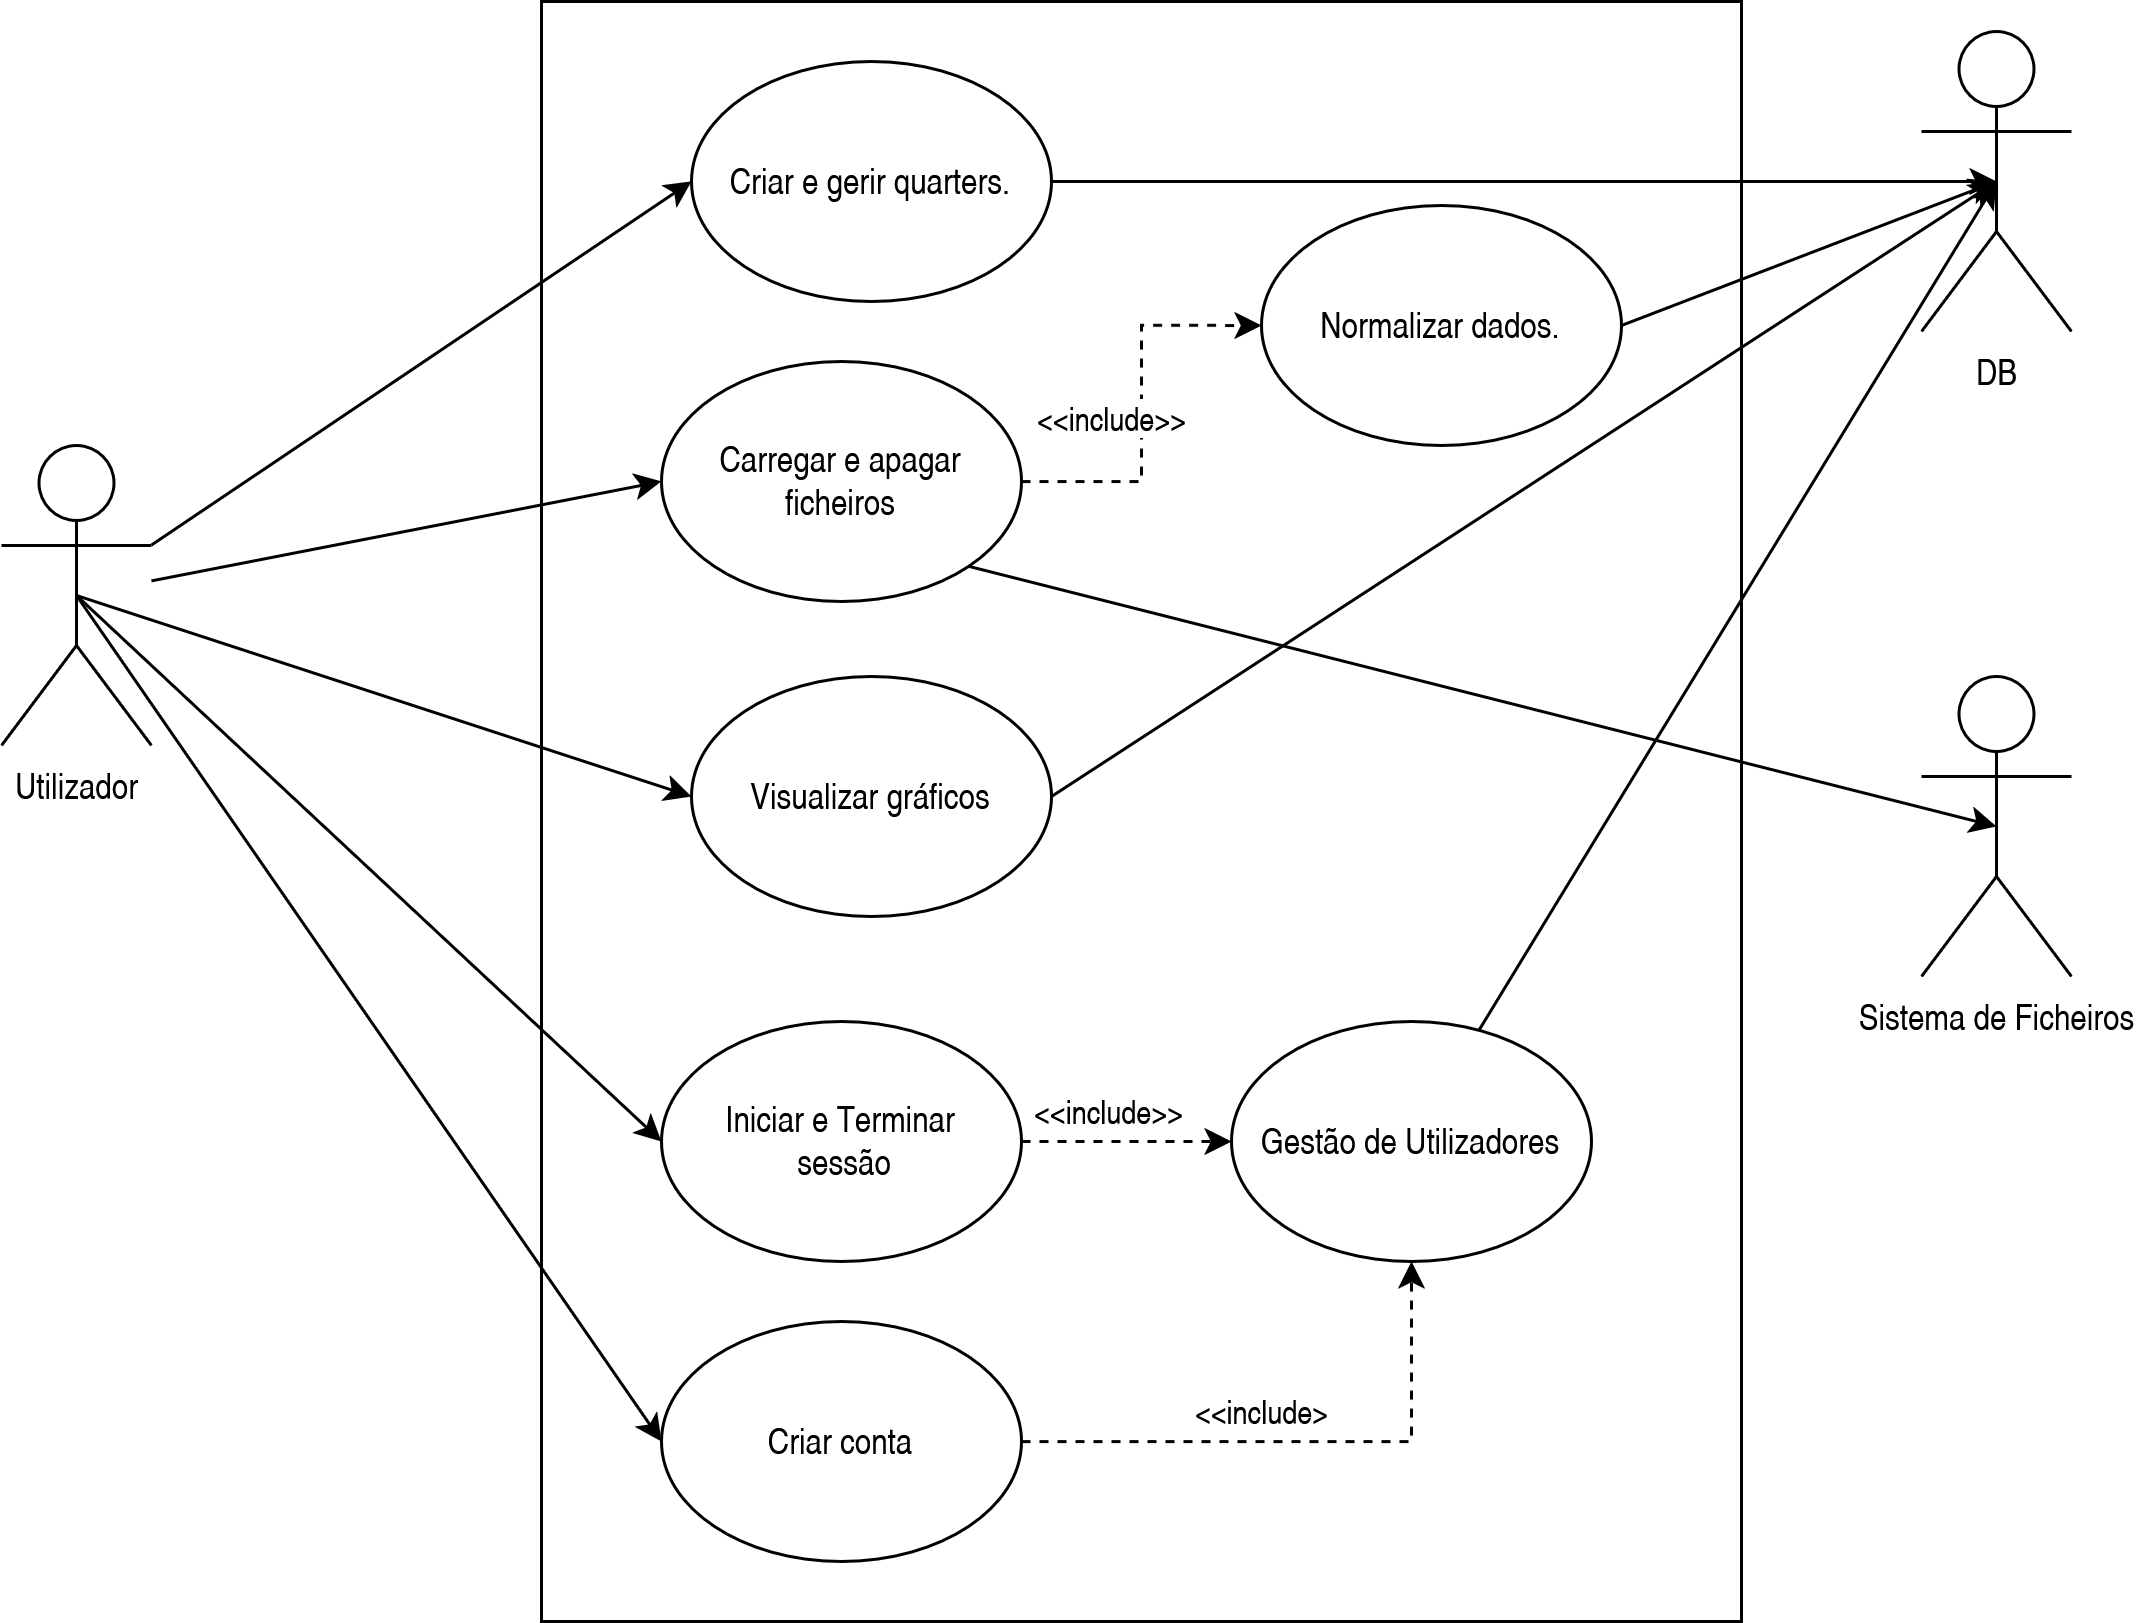
\includegraphics[width=14cm]{./img/usecase_uml}
\caption{\gls{uml} dos Casos de Utilização}
\label{fig:umlCasosUtilizacao}
\end{figure}

A figura~\ref{fig:umlCasosUtilizacao} apresenta o diagrama UML de casos de utilização da aplicação desenvolvida. Este diagrama ilustra as principais interações entre o utilizador e o sistema, bem como a forma como diferentes componentes externos — nomeadamente a base de dados e o sistema de ficheiros — participam nas operações principais da plataforma.

\subsection*{Atores}
\begin{itemize}
    \item \textbf{Utilizador} — É o ator principal, responsável por interagir com o sistema. Pode criar conta, iniciar sessão, carregar ficheiros, visualizar gráficos, entre outras ações.
    \item \textbf{DB (Base de Dados)} — Responsável por armazenar dados estruturados, incluindo utilizadores, trimestres, ficheiros processados e metadados associada.
    \item \textbf{Sistema de Ficheiros} — Componente externo responsável pelo armazenamento físico dos ficheiros carregados e transformados (como por exemplo os ficheiros Excel carregados).
\end{itemize}

\subsection*{Casos de Utilização}
\begin{itemize}
    \item \textbf{Criar e gerir \textit{quarters}} — Permite ao utilizador criar unidades lógicas que agrupam os ficheiros por trimestre. Cada \textit{quarter} é identificado por um \gls{uuid} e guardado na base de dados.
    \item \textbf{Carregar e apagar ficheiros} — Os utilizadores podem carregar ficheiros XLSX para o sistema, que são automaticamente processados. Também podem remover ficheiros já existentes. Esta operação interage com a base de dados e com o sistema de ficheiros.
    \item \textbf{Normalizar dados} (\textit{include}) — Sub-processo chamado sempre que é feito o carregamento de um ficheiro. Este módulo transforma os dados em formato normalizado (por exemplo, convertendo para CSV, limpando colunas inúteis e ajustando nomes). Comunica diretamente com a base de dados e com o sistema de ficheiros.
    \item \textbf{Visualizar gráficos} — Permite ao utilizador consultar representações gráficas dos dados processados, com suporte a filtros e navegação entre trimestres. Os dados são extraídos dos ficheiros normalizados e da base de dados.
    \item \textbf{Iniciar e terminar sessão} — Processo de autenticação e gestão de sessão do utilizador. Este caso inclui o uso do módulo de \textbf{Gestão de Utilizadores}.
    \item \textbf{Criar conta} — Permite a criação de um novo utilizador no sistema, também incluindo a \textbf{Gestão de Utilizadores}.
    \item \textbf{Gestão de Utilizadores} (\textit{include}) — Caso comum que trata a criação, verificação e autenticação de contas de utilizador. Serve de base a outros casos como iniciar sessão ou registar conta.
\end{itemize}

Este diagrama permite compreender de forma clara as funcionalidades principais da plataforma e a separação de responsabilidades entre os diferentes componentes do sistema.

\chapter{Classificação das folhas \gls{xlsx}}


\chapter{Comparação de gráficos suportados pelo \textit{Plotly} e Chart.js}
\label{ch:charts}

\begin{table}[H]
\centering
\caption{Comparação de tipos de gráficos suportados por \textit{Plotly}.js e Chart.js}
\begin{tabular}{|l|c|c|}
\hline
\textbf{Tipo de Gráfico} & \textbf{Plotly.js} & \textbf{Chart.js} \\
\hline
Barras                         & Suportado & Suportado \\
Linhas                         & Suportado & Suportado \\
Dispersão (Scatter)            & Suportado & Suportado \\
Circular (Pie)                 & Suportado & Suportado \\
Área                           & Suportado & Suportado \\
Radar                          & Suportado & Suportado \\
Histograma                     & Suportado & Suportado \\
Box Plot                       & Suportado & Não Suportado \\
Mapa de Calor (Heatmap)        & Suportado & Não Suportado \\
Cascata (Waterfall)            & Suportado & Não Suportado \\
Indicadores (Gauges)           & Suportado & Não Suportado \\
Candlestick (Finanças)         & Suportado & Não Suportado \\
OHLC (Finanças)                & Suportado & Não Suportado \\
Treemap                        & Suportado & Não Suportado \\
Sunburst                       & Suportado & Não Suportado \\
Violin                         & Suportado & Não Suportado \\
Mapa (Geo)                     & Suportado & Não Suportado \\
\hline
\end{tabular}
\label{tab:charts}
\end{table}


\chapter{Pipelines ETL}
\label{ch:etl}

Uma \textit{pipeline} \gls{etl} é um processo utilizado em sistemas de tratamento e integração de dados, com o objetivo de mover dados de uma ou mais fontes para um destino, geralmente uma base de dados ou um sistema de análise. O nome \gls{etl} representa as três etapas principais:

\begin{itemize}
  \item \textbf{Extract (Extração)}: consiste em recolher os dados de múltiplas fontes de informação, que podem incluir bases de dados relacionais, APIs externas, sensores, entre outros. Esta fase preocupa-se com a capacidade de ler dados e de confirmar que são possiveis de extrair.
  
  \item \textbf{Transform (Transformação)}: nesta etapa os dados extraídos são processados e convertidos num formato mais adequado ao destino. Isso pode incluir tarefas como limpeza de dados (remoção de valores nulos ou duplicados), normalização, agregações, mudanças de tipo, ou cálculos. É nesta fase em que se garante a consistência da informação.

  \item \textbf{Load (Carregamento)}: por fim, os dados transformados são inseridos no sistema de destino, normalmente um \textit{data warehouse},  O carregamento é feito dependendo dos requisitos do sistema de destino

\end{itemize}

As \textit{pipelines} \gls{etl} são muito utilizadas em contextos onde há necessidade de consolidar dados de várias origens, permitindo análises mais completas. São fundamentais em áreas como \textit{business intelligence}, ciência de dados e integração de sistemas.

\chapter{Controlo de Versões e GitHub}

O controlo de versões é uma componente essencial em qualquer projeto de desenvolvimento de software, uma vez que permite acompanhar de forma sistemática todas as alterações ao código, colaborar entre vários programadores e garantir a integridade e consistência do código ao longo do tempo.

No contexto deste projeto, o controlo de versões revelou-se particularmente importante para organizar a implementação da plataforma, bem como para permitir uma evolução controlada e iterativa da aplicação, com ciclos de desenvolvimento, testes e correção de erros bem definidos.

Para responder a estas necessidades, foi escolhido o sistema de controlo de versões \textit{Git}, uma ferramenta amplamente utilizada no setor, sendo uma das mais antigas e mais bem suportadas. O \textit{Git} permite criar \textit{branches} de forma simples, o que facilita o desenvolvimento em paralelo de novas funcionalidades sem interferir com a versão principal da aplicação.

Durante o desenvolvimento da plataforma, esta capacidade de criar \textit{branches} foi útil para testar funcionalidades específicas como o processamento assíncrono dos ficheiros, o sistema de autenticação ou o carregamento e normalização automática dos dados. Cada conjunto de funcionalidades foram desenvolvidas de forma isolada, permitindo testes controlados e evitando conflitos no código principal.

Além do \textit{Git}, foi utilizado o \textit{GitHub} como interface principal para alojar o repositório do projeto e gerir a colaboração. O \textit{GitHub} é uma plataforma web que facilita a revisão de código, a gestão de \textit{pull requests} e o acompanhamento de tarefas e problemas. A integração com \textit{Git} é direta, o que permitiu manter o desenvolvimento organizado e acessível a partir de qualquer dispositivo ou ambiente de trabalho.

Após cada \textit{merge} no \textit{GitHub} é corrido um \textit{workflow} que automaticamente atualiza a versão do código que corre dentro da \gls{vps} que usamos para fazer o correr a aplicação (o nosso ambiente de produção) durante o desenvolvimento. Este \textit{workflow} liga-se por \gls{ssh} ao servidor, puxa a última versão do \textit{branch} principal, e re-inicia os \textit{containers} da aplicação, aplicando as alterações aos modelos de dados e aos ficheiros estáticos.

\chapter{Cenários Gherkin}
\label{ch:cenariosGherkin}

\begin{verbatim}
Scenario: Creating an account
    Given I access the page 
    And I don't have an account or logged in
    Then I should see the "Create Account" link
    When I click the "Create Account" link
    Then I should be redirected to the "Create Account" form
    And I should see the username field
    And I should see the password filed
    And I should see the confirm password field
    When I fill that form
    And I click "Save"
    Then I should be redirected to the "Login" page
\end{verbatim}



\begin{verbatim}
Background:
	Given that I have an account

Scenario: Login on the app
	When access the website
	And I am not logged in
	Then I should see the Login page
	And I should see the username field
	And I should see the password filed
	When I fill that form with my login details
	And I click "Save"
	Then I should be redirected to the "Home" page
\end{verbatim}
    
\begin{verbatim}
Background:
	Given that I have an account
	And I am logged in on the application

Scenario: Uploading Q1 files
	When I access the "Uploads" page  
	And I click on "Upload files" button 
	Then the upload modal appears 
	When i click on the upload files box
	And I upload all files from Q1 folder
	And I click "Save"
	Then I should see the files that i just uploaded on the page
	When I navigate to the "Home" page
	Then I should see charts. 
	And I should be able to zoom on the chart
	
Scenario: Uploading Q2 files
	When I access the "Uploads" page  
	And I click on "Upload files" button 
	Then the upload modal appears 
	When i click on the upload files box
	And I upload all files from Q2 folder
	And I confirm that the "Quarter Number" has the value of "2".
	And I click "Save"
	Then I should see the files that i just uploaded on the page
	When I navigate to the "Home" page
	Then I should see charts
	And on the "Customer  Needs" chart, i should be able to navigate to Q1.
	And I should be able to zoom on the chart
\end{verbatim}

\begin{verbatim}
    Background:  
	Given that I have an account
	And I am logged in on the application
	And I have uploaded files to the platform
 
Scenario: Removing a file
	When I navigate to the "Uploads" page  
	Then I should see the files that i already uploaded
	When I click on X button on the file "Customer Needs"
	Then the file is removed from the quarter
	And I should not see charts from that file
	
Scenario: Removing a quarter
	When I navigate to the "Uploads" page  
	Then I should see the files that i already uploaded
	And I should see a "Delete" button.
	When I click on the "Delete" button
	Then I should see all of the files from that section removed 
\end{verbatim}


%%________________________________________________________________________

\bibliographystyle{apalikeMy}
\backmatter
\bibliography{Xbib}


\end{document}
